\chapter{Results}\label{Results}

\section{Evaluation scope}

The verification methodology, vector format and post-processing flow were described in Chapter~\ref{Verification and simulation}. This chapter uses the outputs of that flow to evaluate the implemented carrier-recovery design. The evaluation is organised around three questions:
\begin{itemize}
    \item whether the \ac{RTL} implementation follows the Python reference behaviour closely enough for system-level interpretation,
    \item whether the recovered symbols improve under the residual-\ac{CFO}, linewidth and \ac{SNR} conditions for which the architecture was designed,
    \item and how the selected algorithmic parameters relate to hardware cost, latency and timing.
\end{itemize}

The first part of the chapter therefore checks the main processing blocks against controlled reference cases. The \ac{SBPS} and \ac{SE} blocks are tested with deterministic phase sweeps, while the complete receiver is compared against the floating-point Python model for representative channel cases. The second part evaluates correction quality using constellation diagrams, \ac{EVM} metrics and parameter sweeps.

The main design parameters considered in the sweeps are the number of \ac{SBPS} refinement stages and the number of phase-compensation sections. The residual \ac{CFO} and linewidth are varied to test whether the same hardware settings remain useful as the intra-block phase evolution becomes more demanding. Unless stated otherwise, the same transmitted bit sequence and channel seed are used when comparing parameter settings. This makes the curves directly comparable: differences in the plotted metrics are then caused by the receiver configuration rather than by a different noise realisation.

The default simulation settings are given in Table~\ref{tab:results-case-matrix}. The normalized residual-\ac{CFO} value $\Delta f T_s = 2\times10^{-3}$ corresponds to a residual frequency offset of 64~MHz for the assumed 32~GBd symbol rate. Similarly, the normalized linewidth values used in the sweeps can be converted to physical linewidths by dividing the plotted product $\Delta\nu T_s$ by $T_s = 31.25$~ps. These normalized values are used in the plots because they directly determine the accumulated phase variation per symbol.

\begin{table}[H]
\centering
\caption{Overview of the simulation defaults used for the system-level results}
\label{tab:results-case-matrix}
\begin{tabular}{l l}
\hline
Parameter & Default value \\
\hline
Modulation format & \ac{16QAM}, Gray-coded \\
Block size \(B\) & 32 \\
\ac{SBPS} stages & 6 \\
Radius-directed stages & 2 \\
Phase-compensation sections & 8 \\
\ac{SNR} &  28~dB \\
Residual \ac{CFO} & $\Delta f T_s = 2\times10^{-3}$ \\
Linewidth setting & $\Delta \nu T_s = 3\times10^{-5}$ \\
Number of compared symbols & 6400 per case \\
\hline
\end{tabular}
\end{table}

\section{Agreement with the reference model}

\subsection{SBPS}
The \ac{SBPS} block was first evaluated in isolation using a VHDL testbench that exposes the raw fixed-point cosine and sine outputs of the final refinement stage. The stimulus is a deterministic phase sweep: each symbol in the block is rotated by a known phase offset, and the offset is stepped over the test range. No \ac{AWGN}, linewidth noise or residual-\ac{CFO} variation is added in this block-level test, so the observed error is dominated by the search procedure and fixed-point arithmetic rather than by channel randomness.

Only inner- and outer-ring \ac{16QAM} symbols are used in this idealised test case. This avoids the pattern effect discussed in Section~\ref{sec:Serialized binary phase search}, where middle-ring symbols can create misleading local minima for the decision-directed metric. As a consequence, this isolated test mainly validates the binary phase-search and fixed-point trigonometric output path. It does not by itself validate the radius-directed early stages, because the selected stimulus deliberately avoids the symbols for which that logic is most relevant. The radius-directed path is instead exercised in the top-level comparison of Subsection~\ref{subsec:results-top-level-agreement}.

For this block-level check the testbench uses 12 \ac{SBPS} refinement stages. From Equation~\ref{eq:sbps resolution}, the final correction step is approximately \(0.011^{\circ}\). This is finer than the stage count used in the final receiver, but it is useful for validation because it separates the intended search behaviour from coarse phase-quantisation effects.

Figures~\ref{fig:sbps-cos} and~\ref{fig:sbps-sin} compare the \ac{RTL} trigonometric outputs with the golden reference. The largest relative deviations occur around points where one of the reference components approaches zero, for example the cosine channel near \(\pi/2\). In these regions the relative-error metric is poorly conditioned: a small absolute fixed-point difference is divided by a very small reference value and therefore appears as a visible spike. Away from these zero crossings, the relative error remains below approximately 0.25\%, indicating that the implemented \ac{SBPS} output path follows the expected phase estimate.

\begin{figure}[H]
\centering
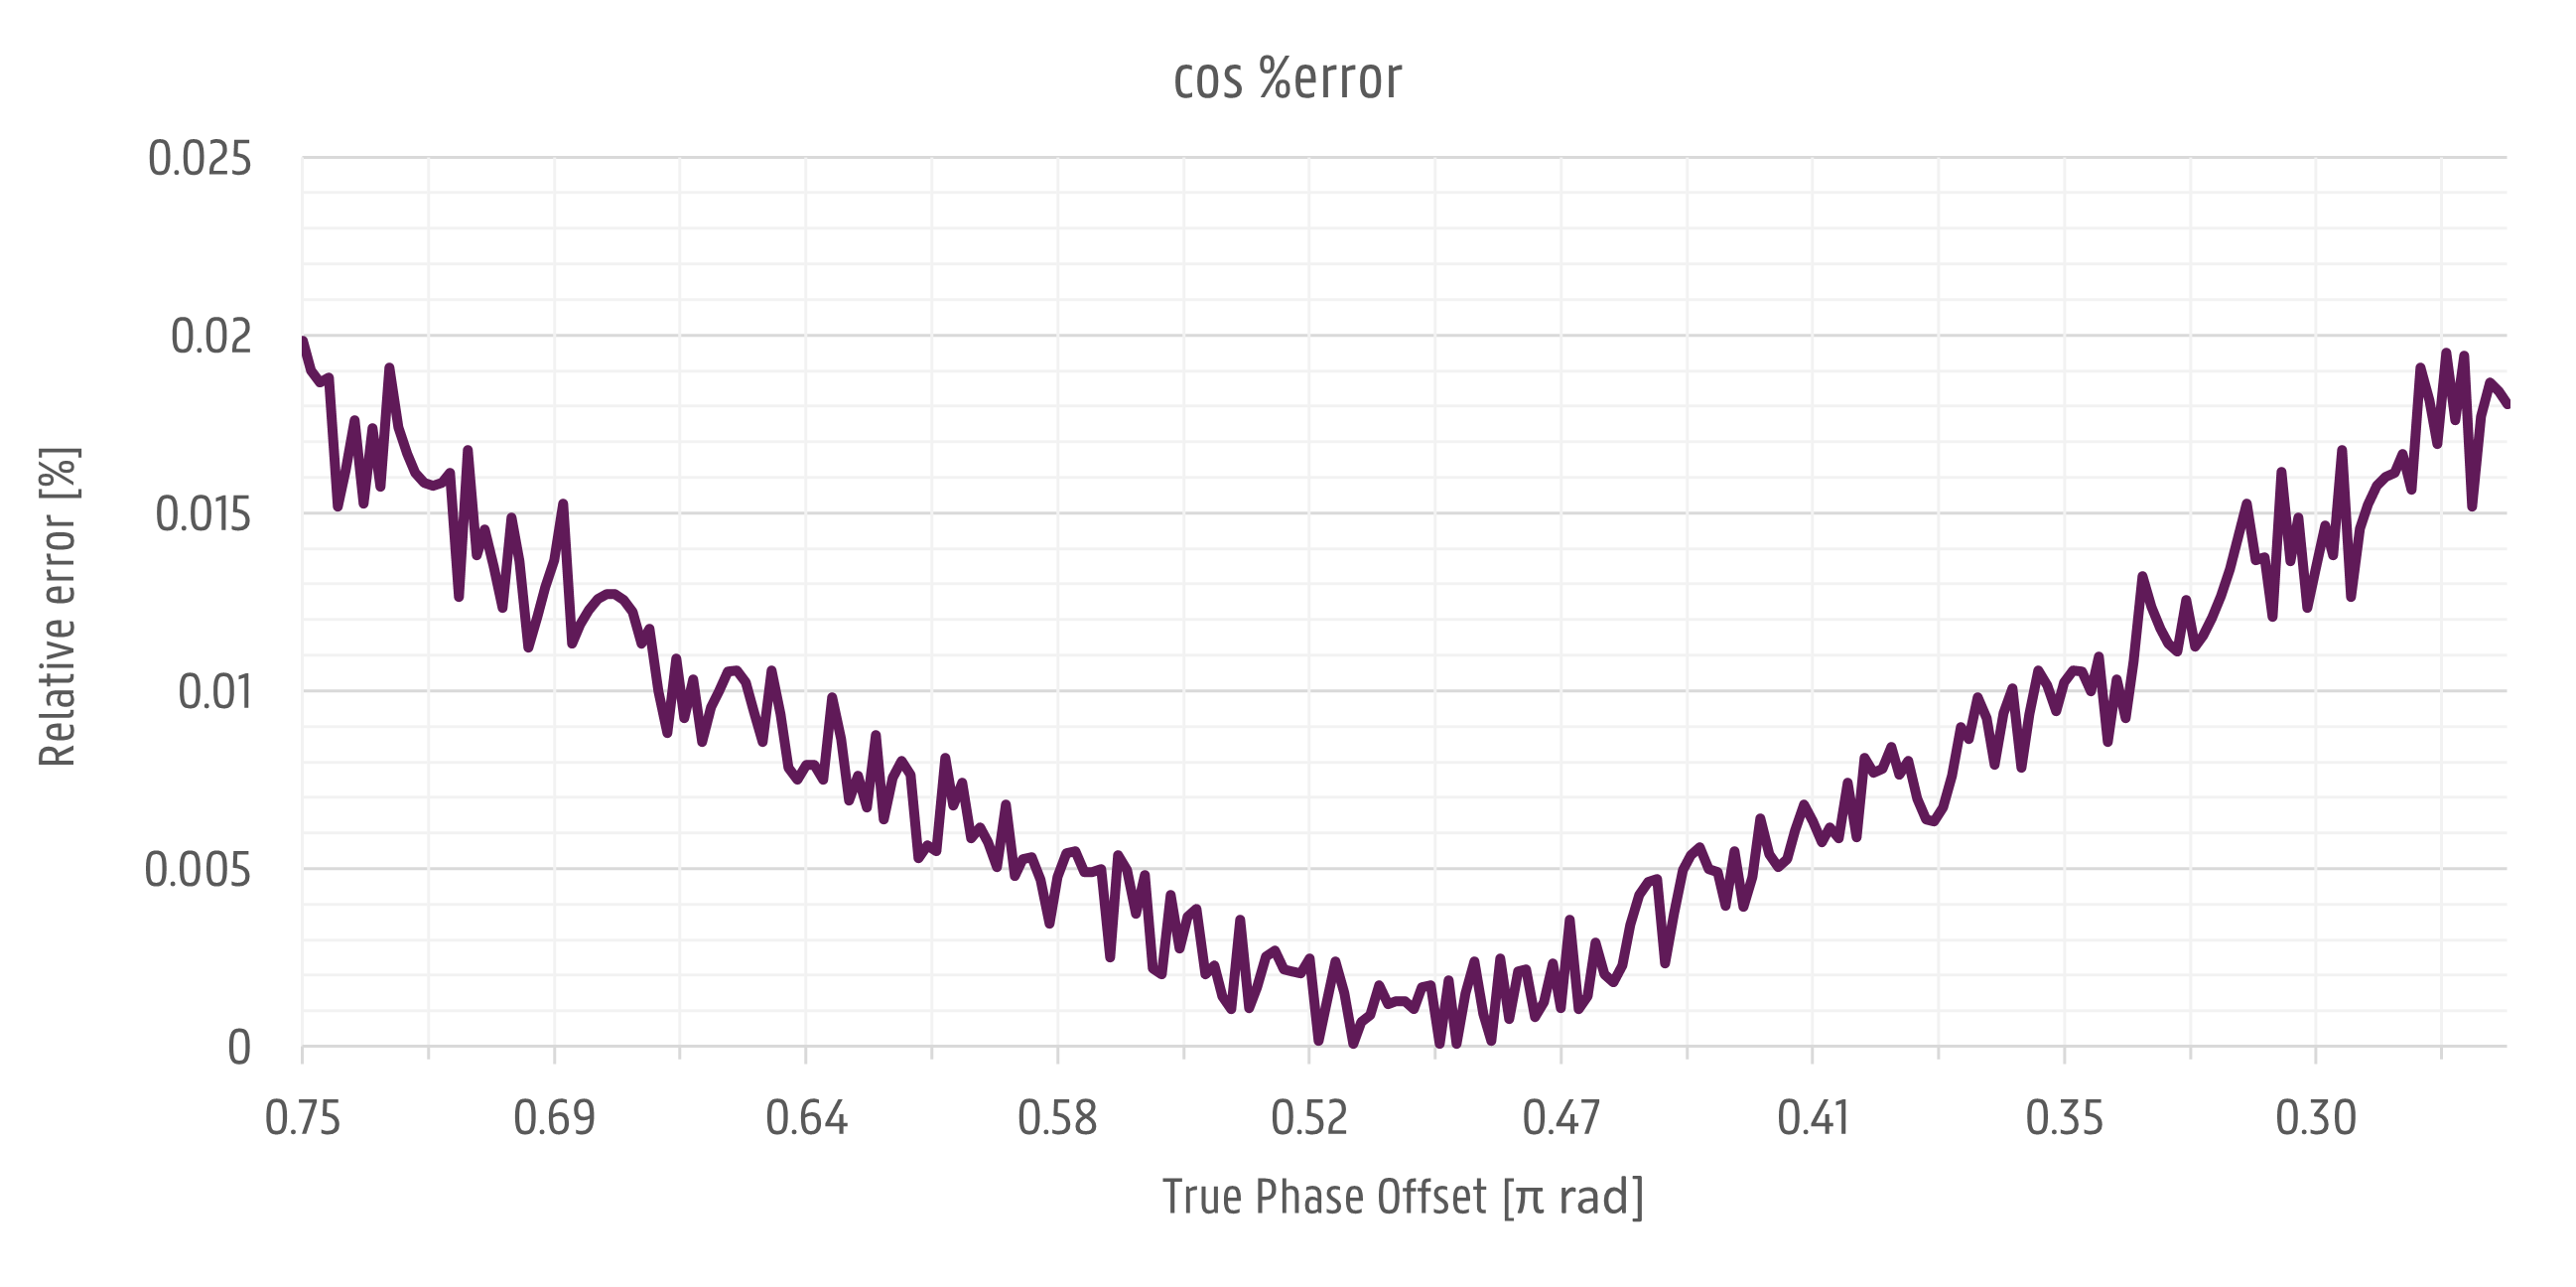
\includegraphics[width=0.8\linewidth]{figures/SBPS_true_phase_RTL_cos.png}
\caption{Relative RTL-cosine error for phase slope}
\label{fig:sbps-cos}
\end{figure}


\begin{figure}[H]
\centering
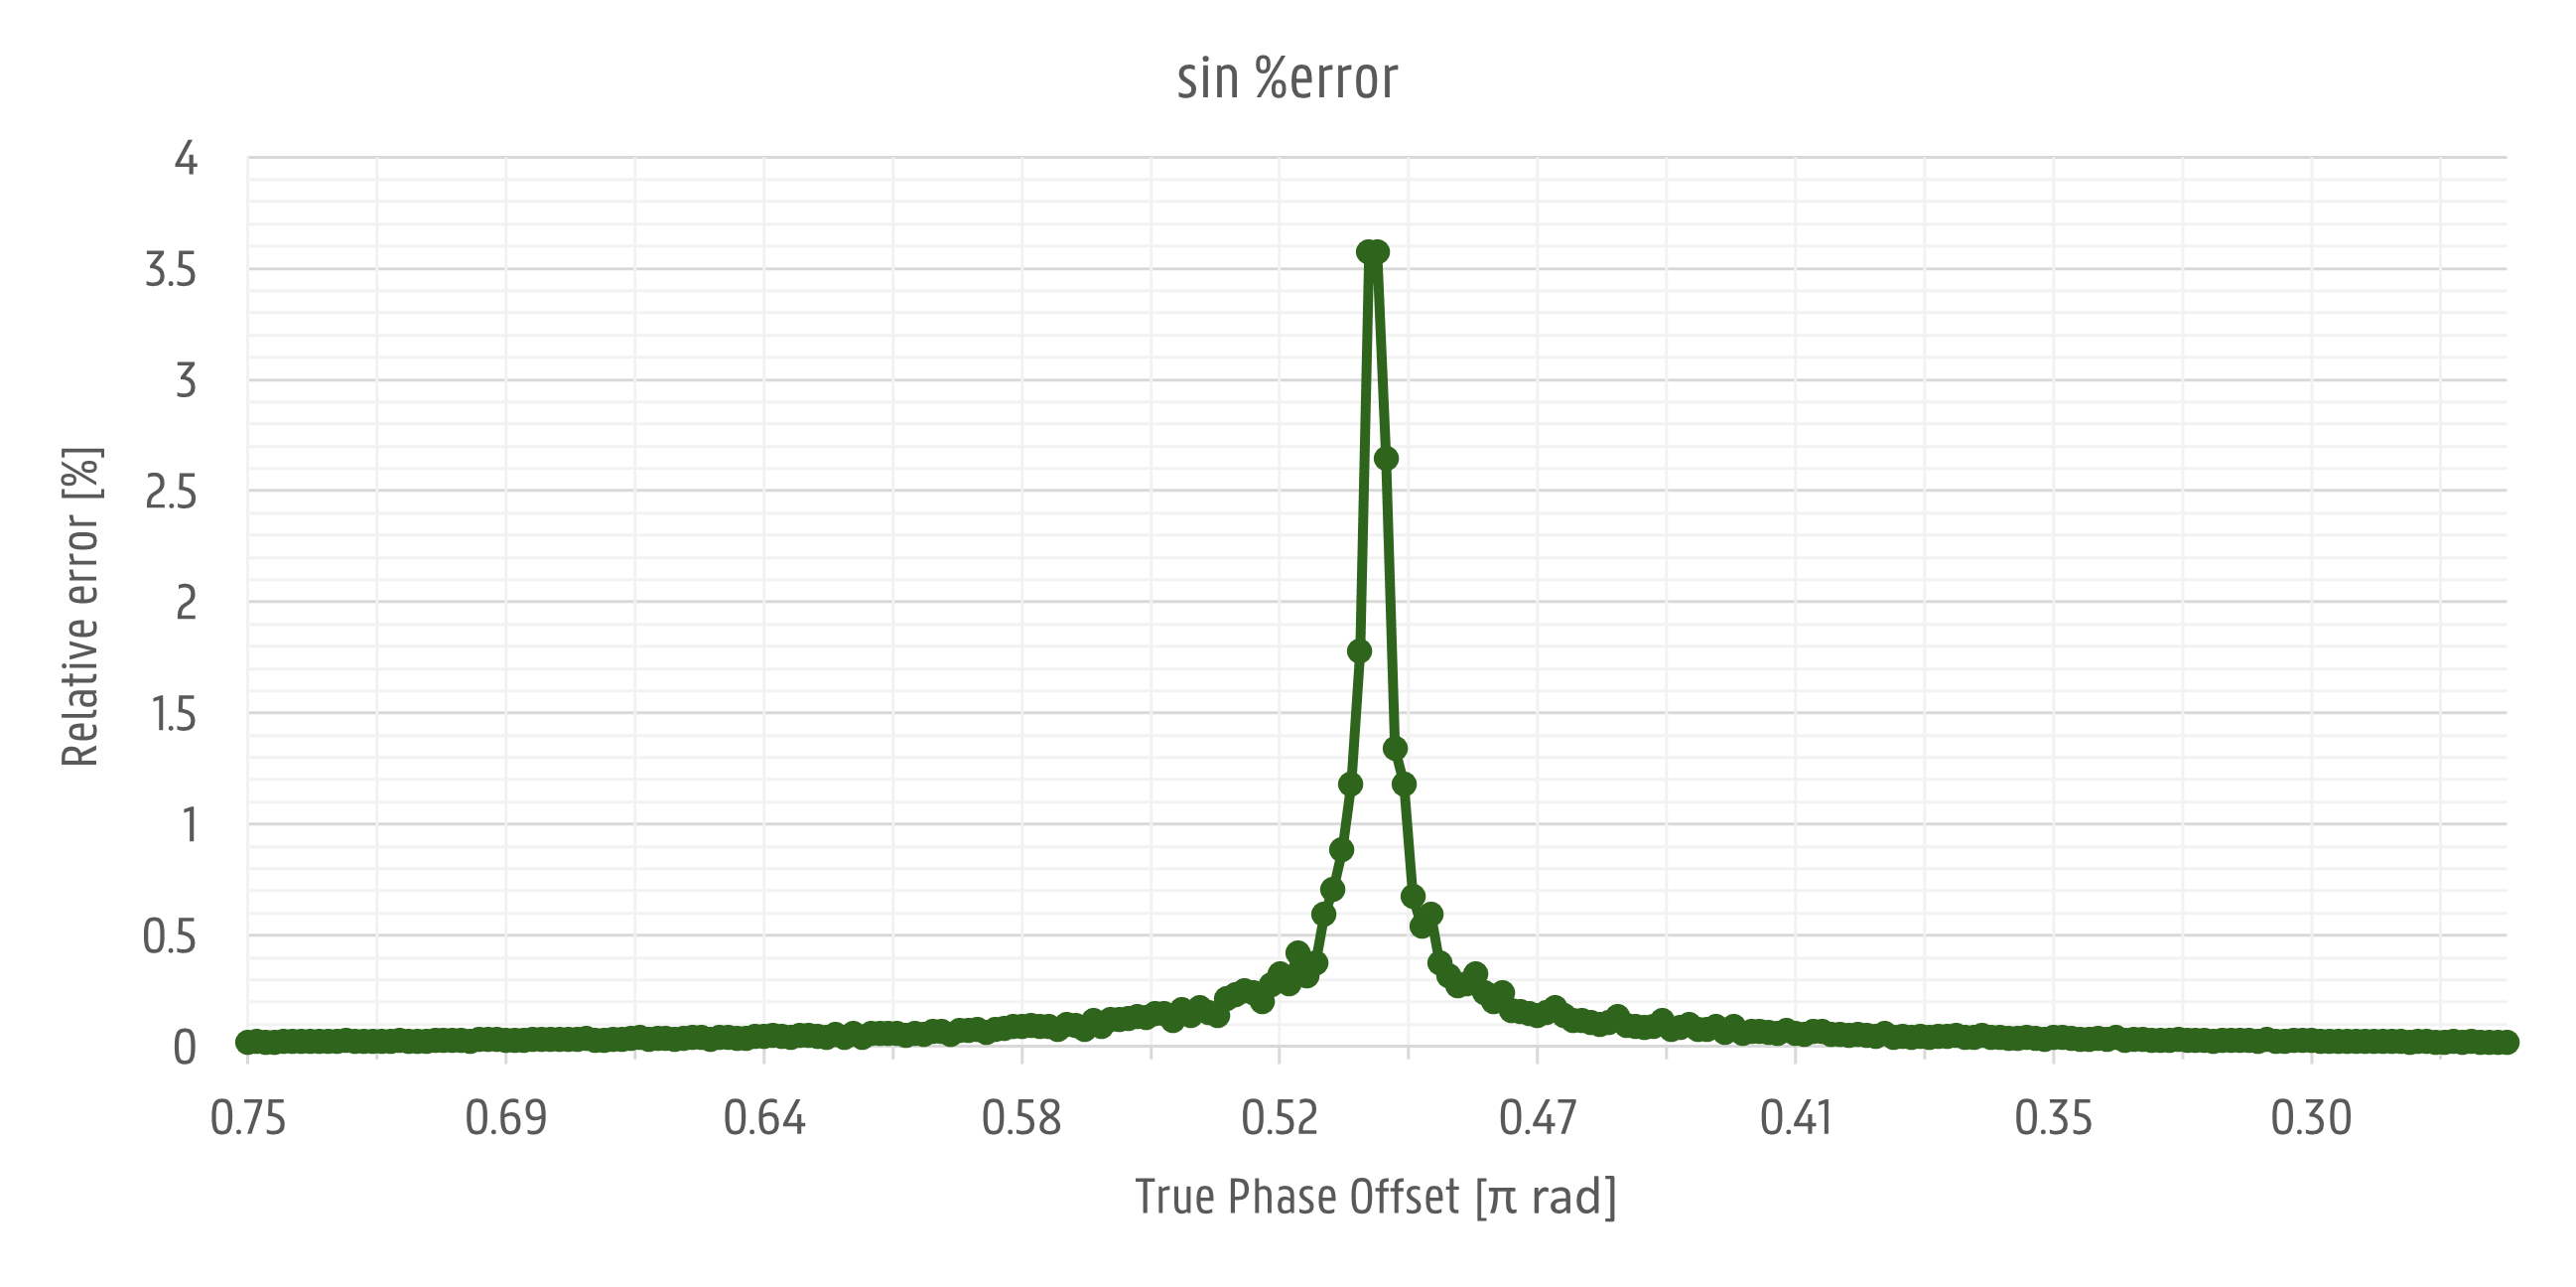
\includegraphics[width=0.8\linewidth]{figures/SBPS_true_phase_RTL_sin.png}
\caption{Relative RTL-sine error for phase slope}
\label{fig:sbps-sin}
\end{figure}

The isolated \ac{SBPS} test therefore supports the functional correctness of the staged phase-search implementation. The remaining deviations are consistent with fixed-point quantisation and with the limitations of a relative-error plot near zero-valued trigonometric components.

\subsection{SE}

For the spread-estimation block, the final \texttt{signed\_theta\_Q428} output is compared against a known intra-block phase sweep over the interval \([-\pi/4,+\pi/4]\). As for the \ac{SBPS} block, the plotted quantity is the relative error with respect to the reference sweep.

This test case is also constructed from inner- and outer-ring symbols only. The spread estimator selects representative symbols near the beginning, middle and end of the block. If a region contains only middle-ring symbols, the selector can legitimately hold the previous valid estimate instead of issuing a new candidate. That behaviour is part of the complete input-selection logic, but it would obscure the numerical accuracy of the spread-estimation datapath in this isolated sweep. The deterministic input selector was therefore verified separately, while Figure~\ref{fig:se-relative error} focuses on the arithmetic path from selected symbols to the signed spread estimate.

\begin{figure}[H]
\centering
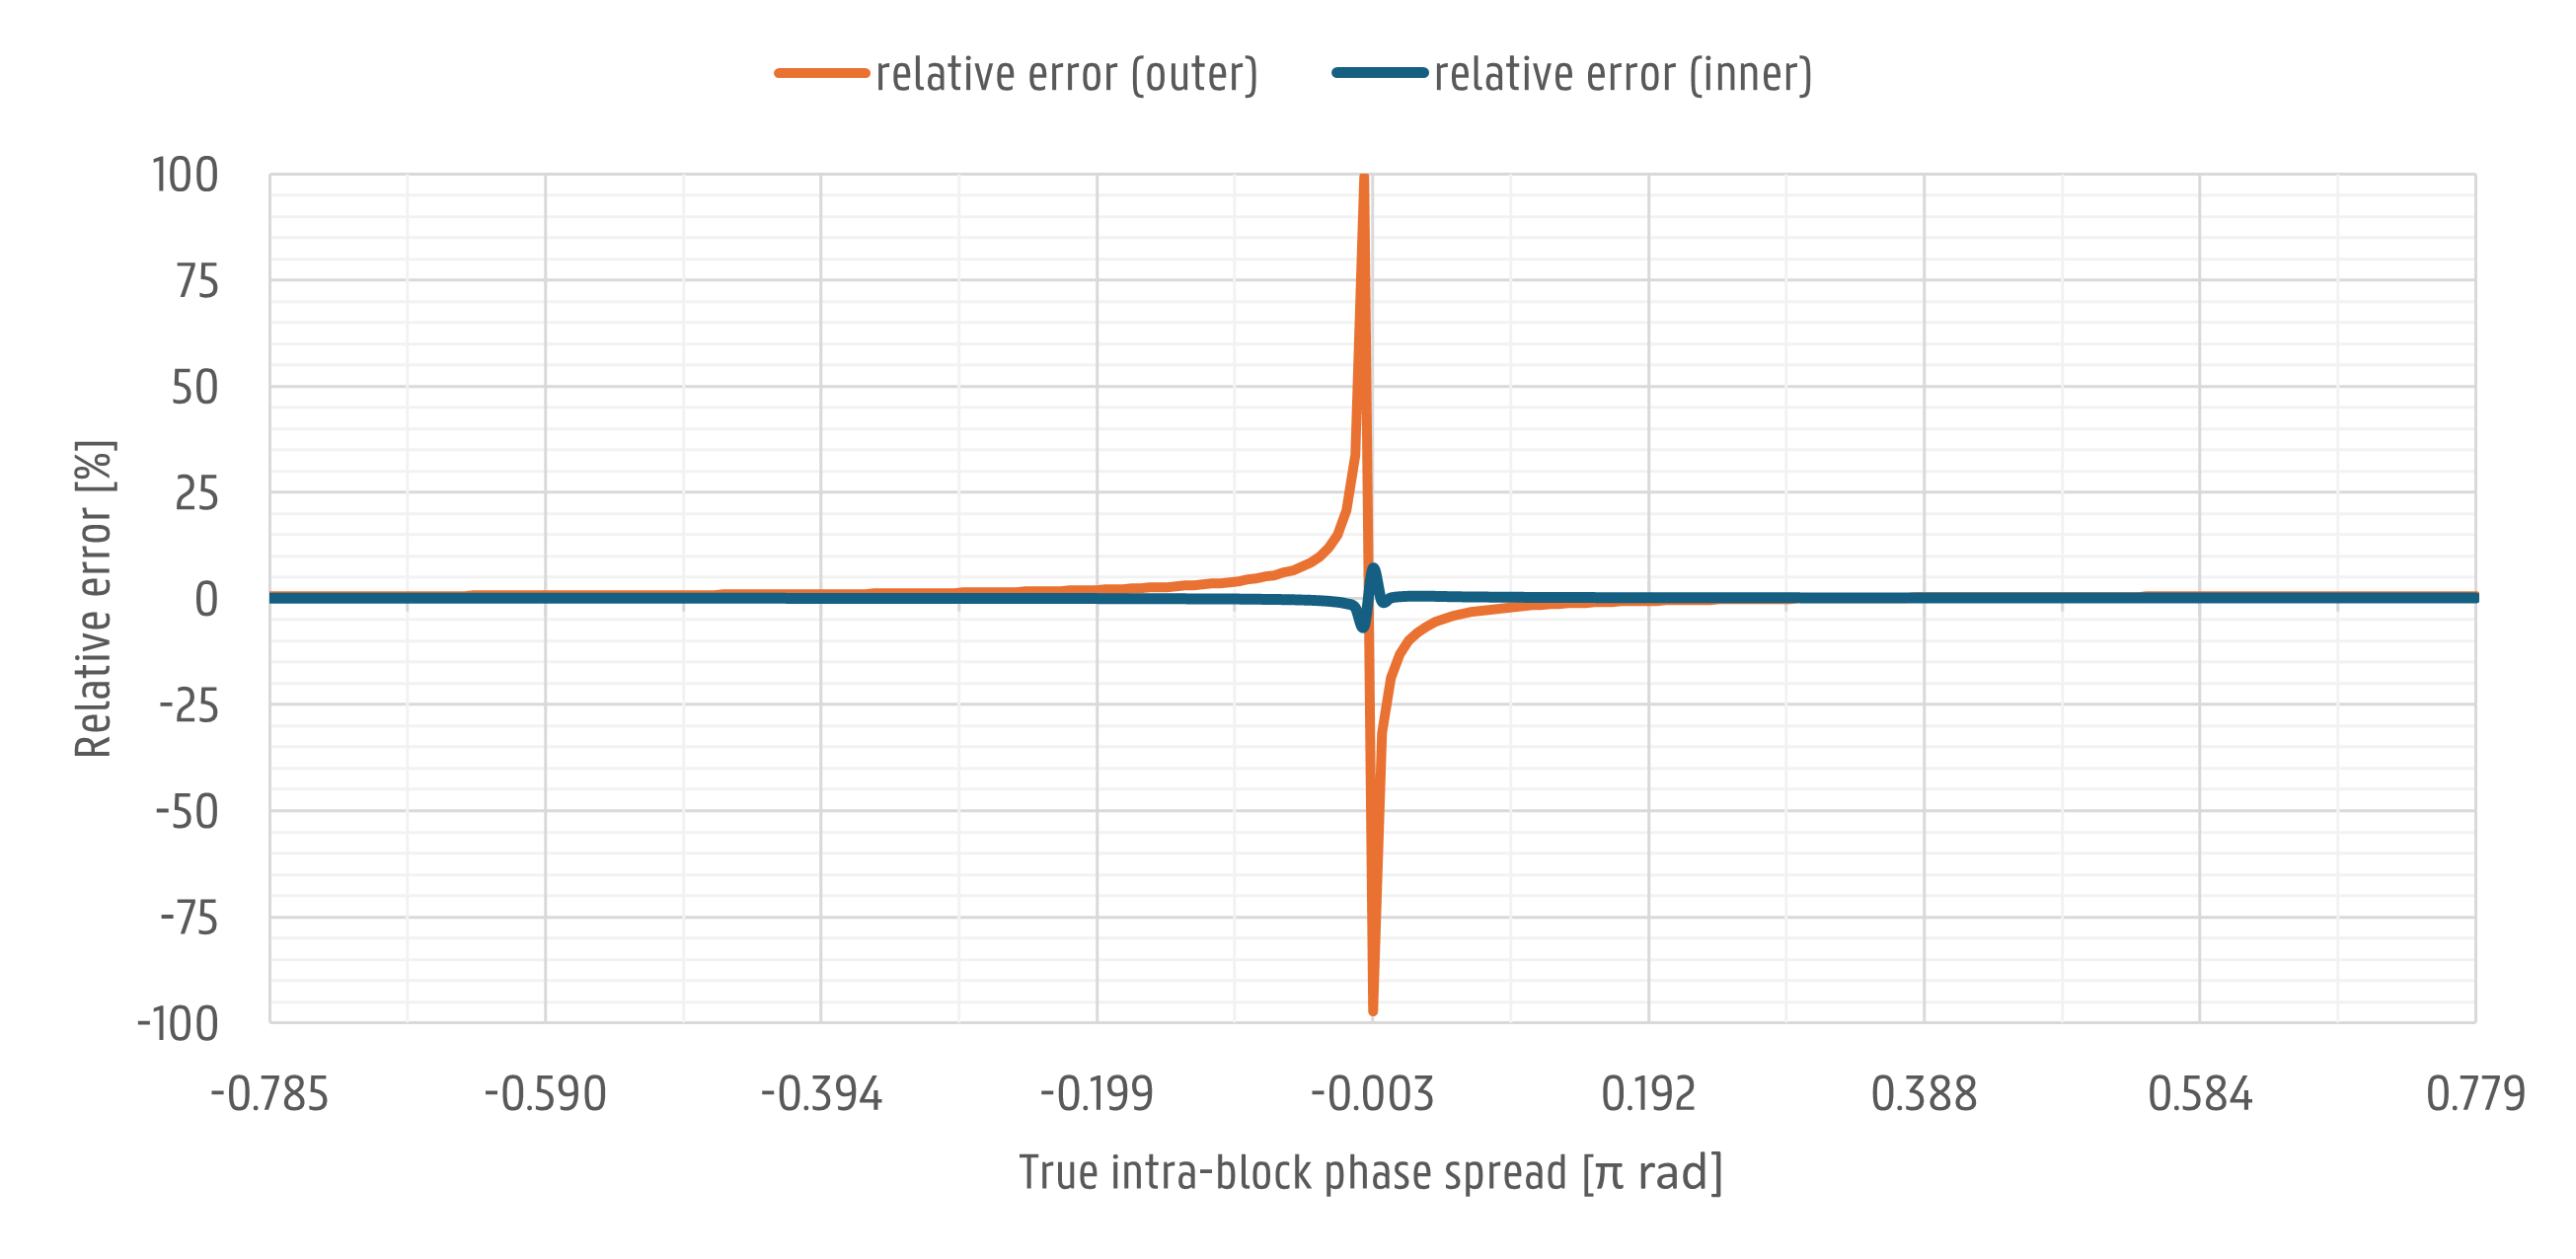
\includegraphics[width=1\linewidth]{figures/SE_true_phase_inner+outer.png}
\caption{Relative RTL error for intra-block phase slope}
\label{fig:se-relative error}
\end{figure}

Figure~\ref{fig:se-relative error} shows that the \ac{RTL} follows the reference over most of the tested interval, with the largest relative deviation concentrated around zero phase spread. This is the least favourable point for a relative-error metric, because the reference angle itself approaches zero. In addition, the normalized dot product approaches \(x=\cos(4|\theta|)=1\), where the \(\arccos(\cdot)\) mapping is highly sensitive to small fixed-point and \ac{LUT}-address quantisation errors. A small absolute error in the normalized cosine can therefore become a large relative error in the recovered angle near zero.

The outer-ring-only case shows the most pronounced zero-spread deviation. This is consistent with the use of a separate outer--outer reciprocal factor in the radius-product normalization: near \(x=1\), even a small fixed-point scaling difference becomes visible after the arccosine conversion. Since the effect is localised around zero spread and does not persist over the full range, it is interpreted as endpoint sensitivity of the fixed-point implementation rather than as a wrong sign decision or a systematic spread-estimation bias.


\subsection{Top-level agreement}\label{subsec:results-top-level-agreement}
Before interpreting the system-level \ac{EVM} curves, the complete fixed-point \ac{RTL} output is compared against the Python reference model. The comparison uses the default receiver configuration from Table~\ref{tab:results-case-matrix}: a block size of 32, six \ac{SBPS} stages, two radius-directed stages and eight compensation sections. Four representative channel cases are evaluated by combining two residual-\ac{CFO} values with two \ac{SNR} values, while the linewidth is kept at the default setting.

The purpose is not to prove that every intermediate integer value is identical, because the two implementations do not use exactly the same arithmetic. Instead, the comparison checks whether the \ac{RTL} produces the same recovered phase behaviour as the reference model within the expected fixed-point error. This also gives an indirect validation of the radius-directed stages. If the radius-directed slicer selected wrong local minima in the early \ac{SBPS} stages, the resulting centre-phase estimate would differ strongly from the Python model and would appear as a large phase-error difference after compensation.

For each model, the phase error is calculated against the clean reference trajectory. The model difference is then computed as:
\begin{equation}
    \Delta \mathrm{ERR} = \mathrm{ERR}_{\mathrm{py}} - \mathrm{ERR}_{\mathrm{RTL}}
\end{equation}

where

\begin{equation}
    \begin{aligned}
        \mathrm{ERR}_{m}
        &=
        \frac{1}{N}
        \sum_{k=0}^{N-1}
        e_{m,k},
        \\
        e_{m,k}
        &=
        \phi_{k,\mathrm{ref}}
        -
        \hat{\phi}_{k,m},
        \qquad
        m \in \{\mathrm{py},\mathrm{RTL}\}.
    \end{aligned}
\end{equation}

Figure~\ref{fig:results-phase-model-rtl} shows this signed model difference as a function of block index for the four residual-\ac{CFO}/\ac{SNR} combinations. The traces fluctuate around zero and do not show a persistent drift over the simulated blocks. This is important, because a systematic offset between the Python model and the \ac{RTL} would indicate either a scaling mismatch, a sign convention error or a fixed delay error in one of the phase paths.

\begin{figure}[H]
\centering
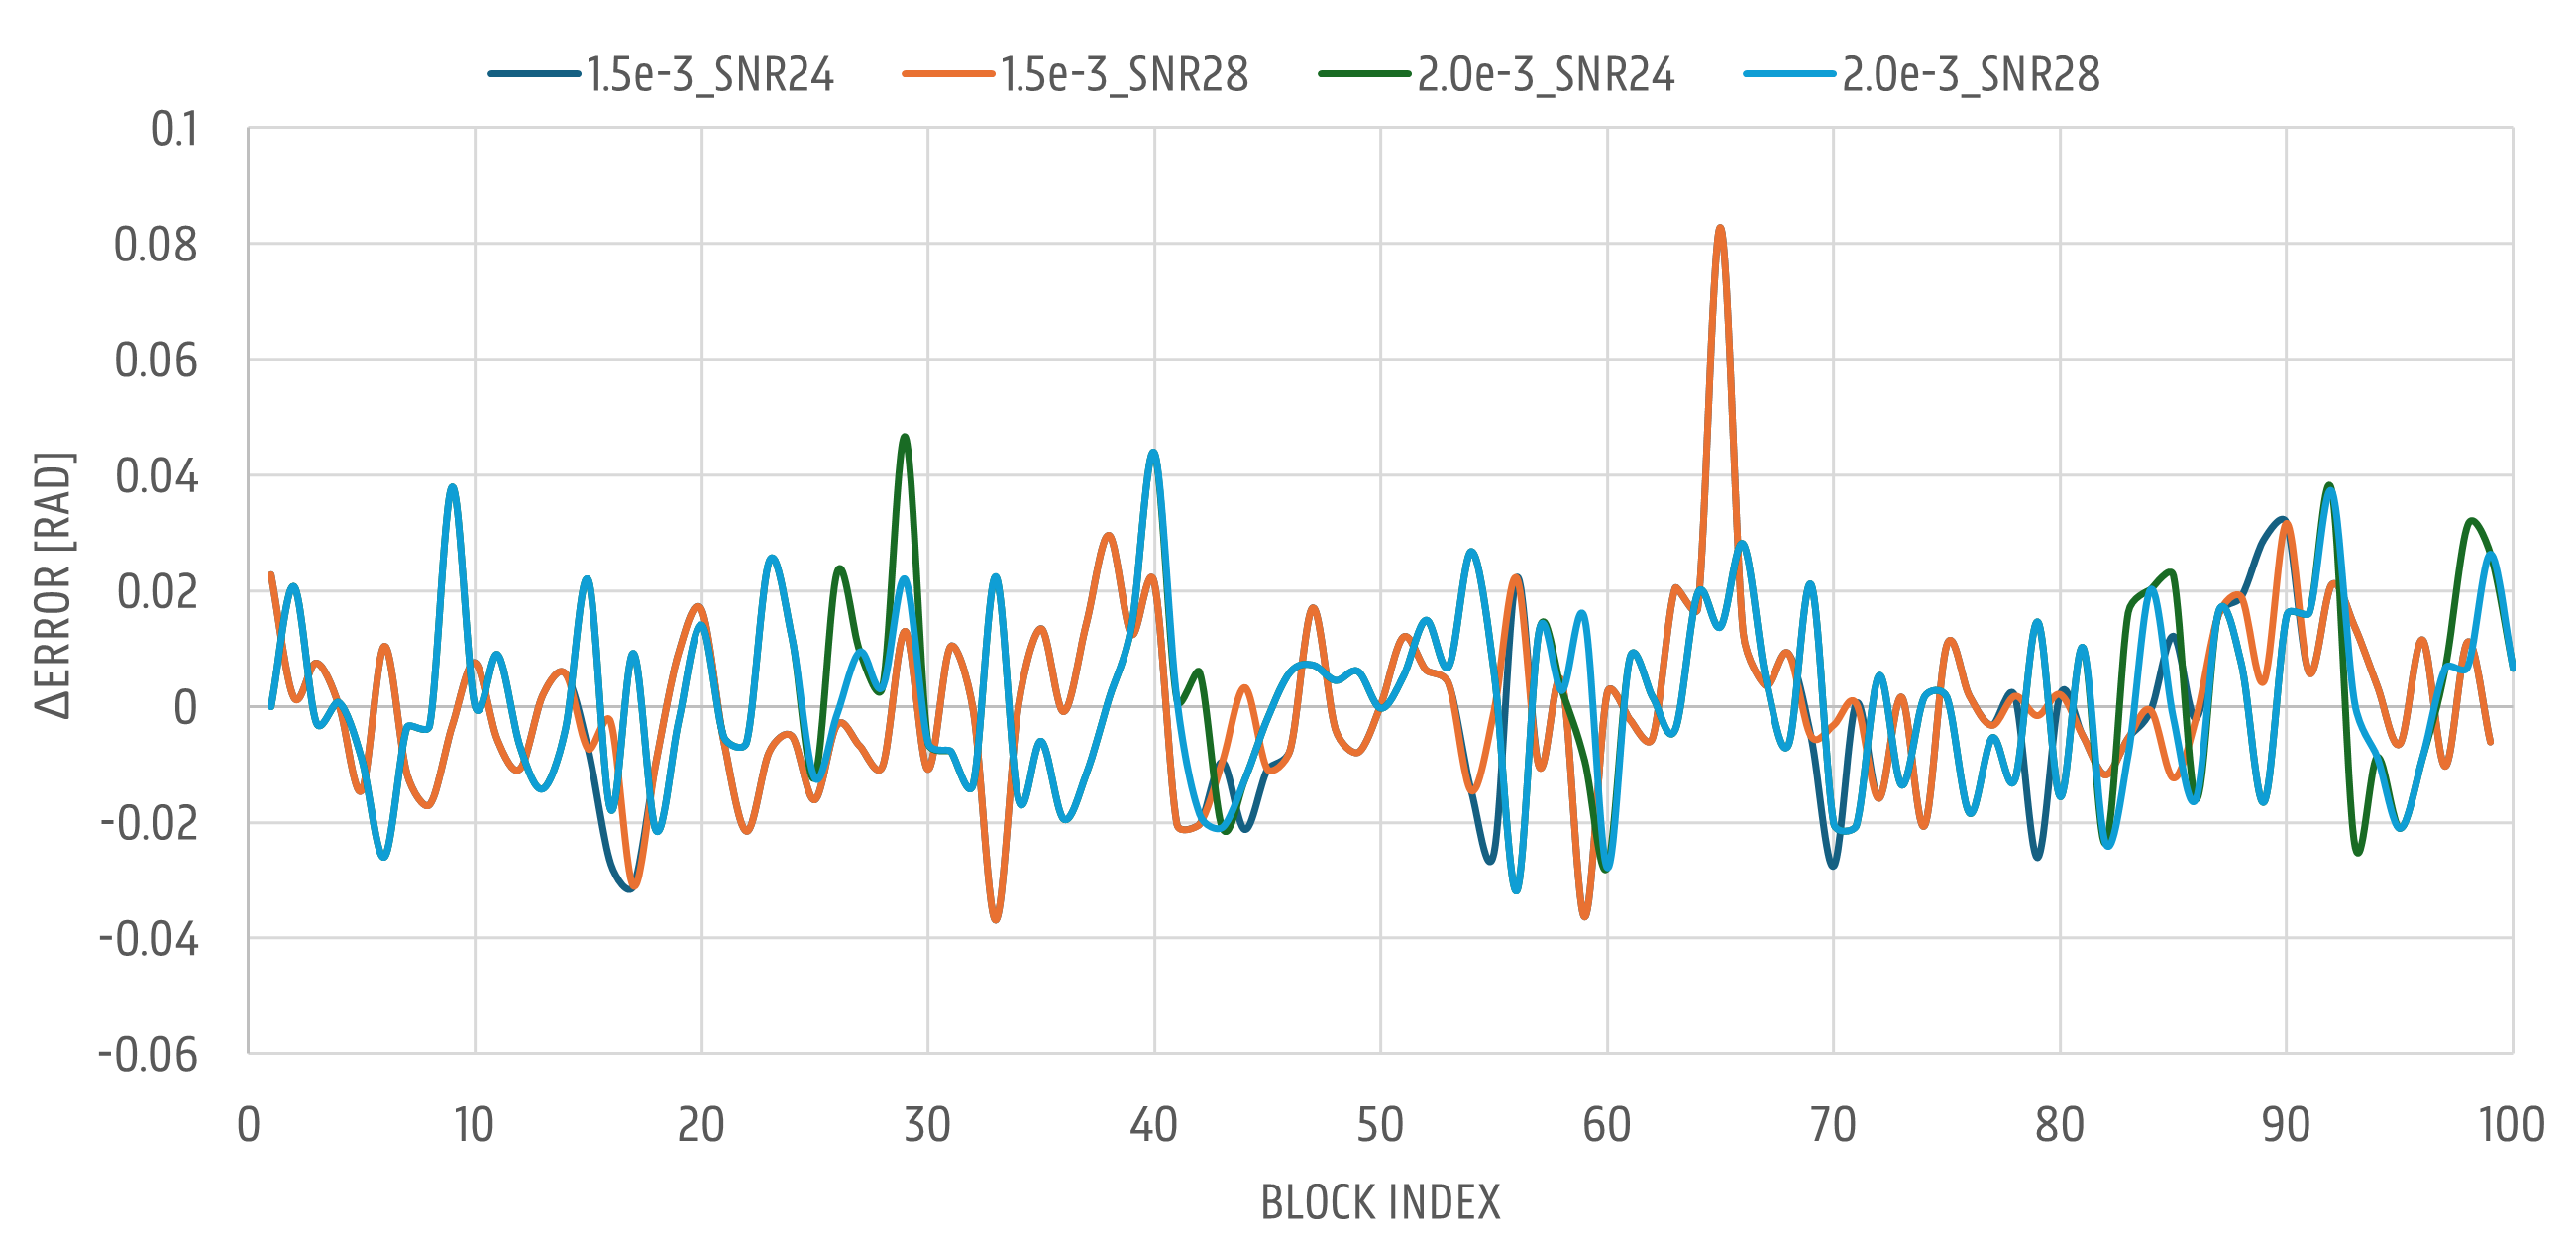
\includegraphics[width=1\linewidth]{figures/error_localisation.png}
\caption{Signed phase-error difference between Python reference model and RTL output over block index}
\label{fig:results-phase-model-rtl}
\end{figure}

The visual observation is confirmed by Table~\ref{tab:model-differences}. For all four cases, the 95\% confidence interval of the mean model difference includes zero. The largest mean offset is 2.251~mrad, which is small compared with the phase drift that must be compensated inside one block.

\begin{table}[H]
\centering
\caption{Python-to-RTL phase-error differences for the top-level receiver, \(n=99\) blocks}
\label{tab:model-differences}
\begin{tabular}{lllll}
\hline
CFO ($\Delta f T_s$) & SNR (dB) & Mean Error {[}mrad{]} & std dev {[}mrad{]} & 95\% CI {[}mrad{]}    \\ \hline
$2e-3$               & 24       & +2.251                & 16.590             & {[}-1.058, +5.559{]}  \\
$2e-3$               & 28       & +1.254                & 16.590             & {[}-1.823, + 4.332{]} \\
$1.5e-3$             & 24       & -0.070                & 16.722             & {[}-3.405, +3.265{]}  \\
$1.5e-3$             & 28       & +0.672                & 15.419             & {[}-2.403, +3.747{]}
\end{tabular}
\end{table}

The remaining difference is consistent with the implementation differences between both models. The Python reference uses floating-point arithmetic, while the \ac{RTL} uses fixed-point quantisation throughout the datapath. In addition, the Python model evaluates the arccosine operation with the NumPy implementation, whereas the \ac{RTL} uses the \ac{LUT}-based approximation described in Subsection~\ref{subsec:spread-estimation}. The final compensation rotation is also not identical: the \ac{RTL} uses a CORDIC-based rotator, while the Python model uses floating-point complex exponentials. Finally, the phase-compensation section coefficients are quantised in the hardware implementation. In the \ac{RTL}, the phase applied to section \(n\) follows
from Equation~\ref{eq:comp_sections}, while the Python model uses the exact floating-point coefficients.

The relative size of the observed model difference can be estimated from the most demanding comparison case, with $\Delta f T_s = 2\times10^{-3}$ and \ac{SNR}~=~24~dB. The deterministic phase increment per symbol due to residual \ac{CFO} is

\begin{equation}
    \Delta \Phi  = 2\pi\Delta f T_s = 12.57~\text{mrad/symbol}.
\end{equation}

For a block of 32 symbols, this corresponds to an intra-block phase change of approximately 0.39~rad, or 22.3 degrees. The largest mean model difference in Table~\ref{tab:model-differences} is therefore below 1\% of the deterministic phase drift across the block. This does not remove the need to consider fixed-point deviations, as the standard deviations are larger than the means, but it does show that the implemented \ac{RTL} does not introduce a measurable average phase bias relative to the reference model.

This agreement validates the use of the \ac{RTL} output in the following sections. The subsequent performance trends can therefore be interpreted as consequences of the algorithmic parameters and channel conditions, rather than as artefacts of a gross mismatch between the reference model and the hardware implementation.

% \subsection{Phase-spread estimation}

% The phase-spread estimator is evaluated separately because it determines how much intra-block phase slope is compensated after the centre phase has been recovered. Figure~\ref{fig:results-spread-model-rtl} should compare the estimated spread from the reference model and the \ac{RTL}. A second panel should show the signed spread-estimation error, preferably in radians and, where relevant, in the corresponding fixed-point \ac{LSB} scale.

% \begin{figure}[H]
% \centering
% \missingfigure{Python versus RTL signed phase-spread estimate, with spread-error subplot.}
% \caption{Reference-model and RTL phase-spread estimates over block index}
% \label{fig:results-spread-model-rtl}
% \end{figure}

\section{Correction behaviour}

This section shows how the recovered signal evolves through the complete carrier-recovery chain. The purpose is to make the separate contributions of the centre-phase estimate and the phase-spread compensation visible before reducing the result to a single \ac{EVM} number.

Figure~\ref{fig:results-constellation-before-after} compares the impaired input, the output after \ac{SBPS}-only correction and the output after combined \ac{SBPS}+\ac{SE} correction for the default case. The left constellation shows the impaired symbols before carrier recovery. The three visible rings correspond to the three possible magnitudes of the normalized \ac{16QAM} constellation. Because the residual \ac{CFO} rotates the constellation over time, and the linewidth adds random phase perturbations, these magnitude classes appear as circular traces rather than as compact decision regions.

The middle constellation shows the effect of applying only the \ac{SBPS} centre-phase estimate. In the \ac{RTL} configuration this corresponds to using one compensation section, so every symbol in the block is rotated by the same unwrapped centre phase. The \ac{SBPS} estimate already removes the dominant common phase rotation: the sixteen decision regions become visible again, and the received symbols are grouped around the ideal constellation points. However, the clusters remain elongated along a rotational direction. This residual spread is expected, because a single centre-phase estimate cannot compensate the phase slope that accumulates between the centre and the edges of the block.

\begin{figure}[H]
\centering
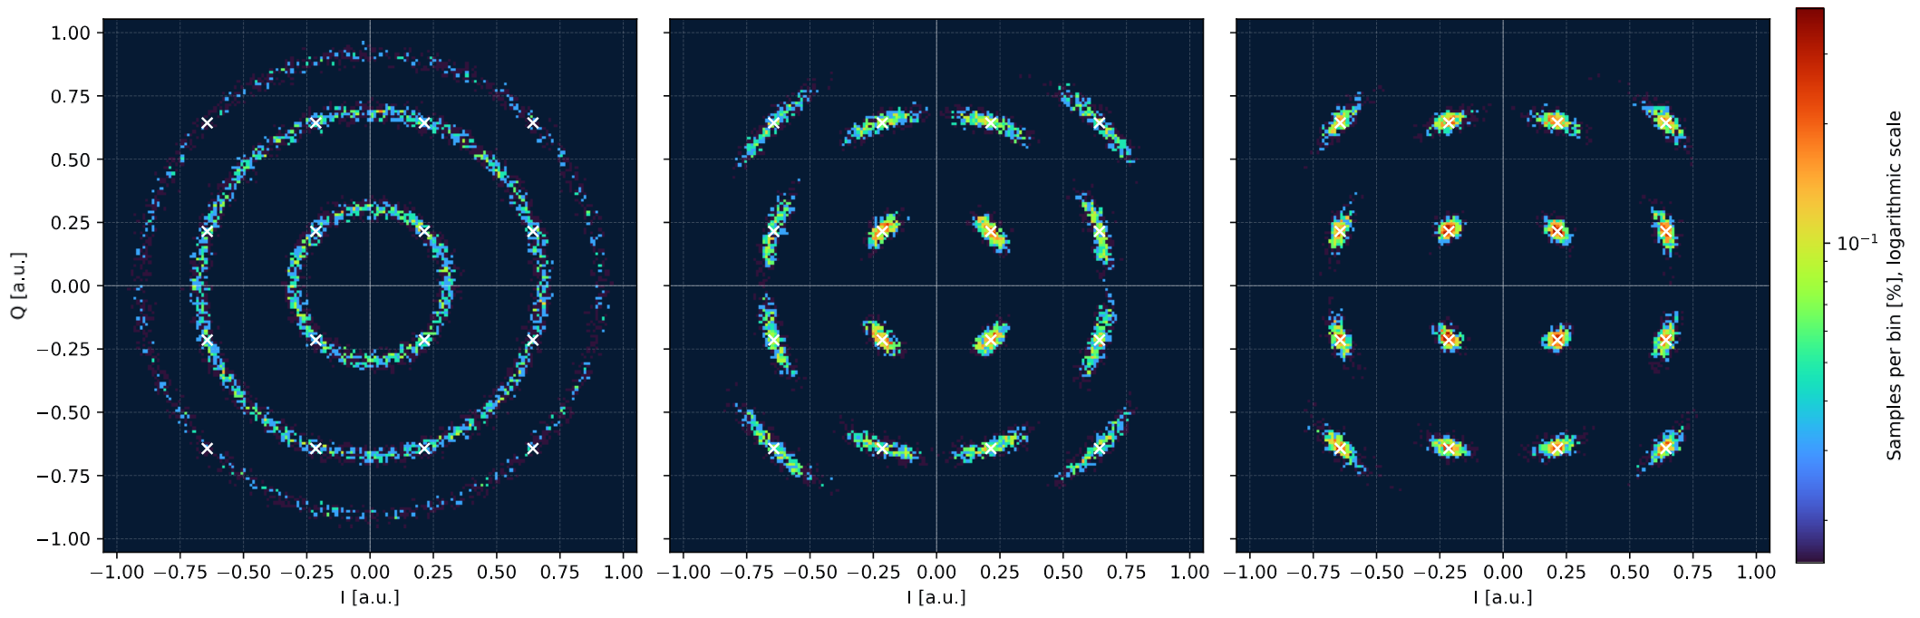
\includegraphics[width=1\linewidth]{figures/block32_cfo64M_constellation_triptych.png}
\caption{Constellation diagram throughout the recovery pipeline}
\label{fig:results-constellation-before-after}
\end{figure}

The right constellation shows the default configuration, where the spread estimate is applied over eight compensation sections across the 32-symbol block. The remaining clusters are visibly more compact than in the \ac{SBPS}-only case, especially for the outer constellation points where a given phase error produces a larger absolute \ac{I/Q} displacement.

The \ac{EVM} values quoted for this comparison are calculated by comparing each observed symbol stream with the corresponding clean transmitted \ac{16QAM} symbols:
\begin{equation}
    \mathrm{EVM}~[\%]
    =
    100
    \sqrt{
    \frac{
    \sum_{k=0}^{N-1}
    \left|r_k - s_k\right|^2
    }{
    \sum_{k=0}^{N-1}
    \left|s_k\right|^2
    }}
    ,
    \label{eq:results-evm-percent}
\end{equation}
where $r_k$ is either the impaired input, the \ac{SBPS}-only output or the \ac{SBPS}+\ac{SE} output, and $s_k$ is the corresponding clean reference symbol. The denominator normalizes the error to the average reference-symbol power, so the result can be reported as a percentage. With this definition, the impaired input has an \ac{EVM} of 142\%, the \ac{SBPS}-only correction reduces it to 12.69\%, and the combined \ac{SBPS}+\ac{SE} correction reduces it further to 7.41\%.

The constellation plots are useful for detecting gross correction behaviour, but they do not fully characterize cycle slips. For square \ac{QAM}, a wrong quadrant branch can rotate the constellation by a multiple of $\pi/2$, which may still look visually plausible in a scatter plot. The remaining sections therefore use \ac{EVM} and symbol-index localisation to distinguish ordinary residual phase error from edge-related compensation limits.

\section{Performance sweeps}\label{sec:results-performance-sweeps}

% The performance sweeps use \ac{BER}, \ac{SER}, \ac{EVM} and residual phase statistics. \ac{BER} is the final communication metric, while \ac{EVM} and residual phase are included because they are more stable for short simulation runs and make it easier to identify the source of a performance change.
The performance sweeps evaluate the two main complexity parameters of the receiver: the number of \ac{SBPS} refinement stages and the number of compensation sections. The primary metric is the relative \ac{EVM} reduction, denoted here as $\Delta\mathrm{EVM}_{\mathrm{dB}}$. This metric is used because it is more stable than \ac{BER} for the short simulation runs used in the parameter sweeps, while still reflecting how much closer the recovered symbols are to the clean reference constellation.

For each case, the input \ac{EVM} is calculated against the clean transmitted symbols before carrier recovery, and the output \ac{EVM} is calculated against the same reference after recovery. The plotted metric is
\begin{equation}
    \Delta\mathrm{EVM}_{\mathrm{dB}}
    =
    20\log_{10}
    \left(
    \frac{\mathrm{EVM}_{\mathrm{out}}}{\mathrm{EVM}_{\mathrm{in}}}
    \right).
    \label{eq:delta-evm}
\end{equation}
With this definition, a more negative value means a larger \ac{EVM} reduction. The shaded multiplier count in the sweep figures gives a first-order indication of the corresponding hardware cost. It is not a complete post-synthesis resource report, but it shows the expected scaling trend as stages or sections are added.


% \subsection{BER versus SNR for residual CFO}

% Figure~\ref{fig:results-ber-snr-cfo} shows the end-to-end \ac{BER} as a function of \ac{SNR}, with one curve for each residual-\ac{CFO} setting. This is the main system-level performance plot. A successful implementation should show that the wrapper maintains the expected \ac{BER} trend over the intended residual-\ac{CFO} range and that the penalty increases when the intra-block phase slope becomes too large for the selected block size and compensation configuration.

% \begin{figure}[H]
% \centering
% \missingfigure{BER versus SNR, grouped by residual CFO.}
% \caption{End-to-end BER versus SNR for different residual-CFO values}
% \label{fig:results-ber-snr-cfo}
% \end{figure}

\subsection{Influence of SBPS refinement stages}

The number of \ac{SBPS} stages determines both the phase-search resolution and the amount of hardware required by the serialized search chain. Figure~\ref{fig:results-ber-stages-cfo} shows the effect of the refinement depth on $\Delta\mathrm{EVM}_{\mathrm{dB}}$ for several linewidth settings. In this sweep, the residual \ac{CFO} is kept at the default value while the linewidth is varied.

\begin{figure}[H]
\centering
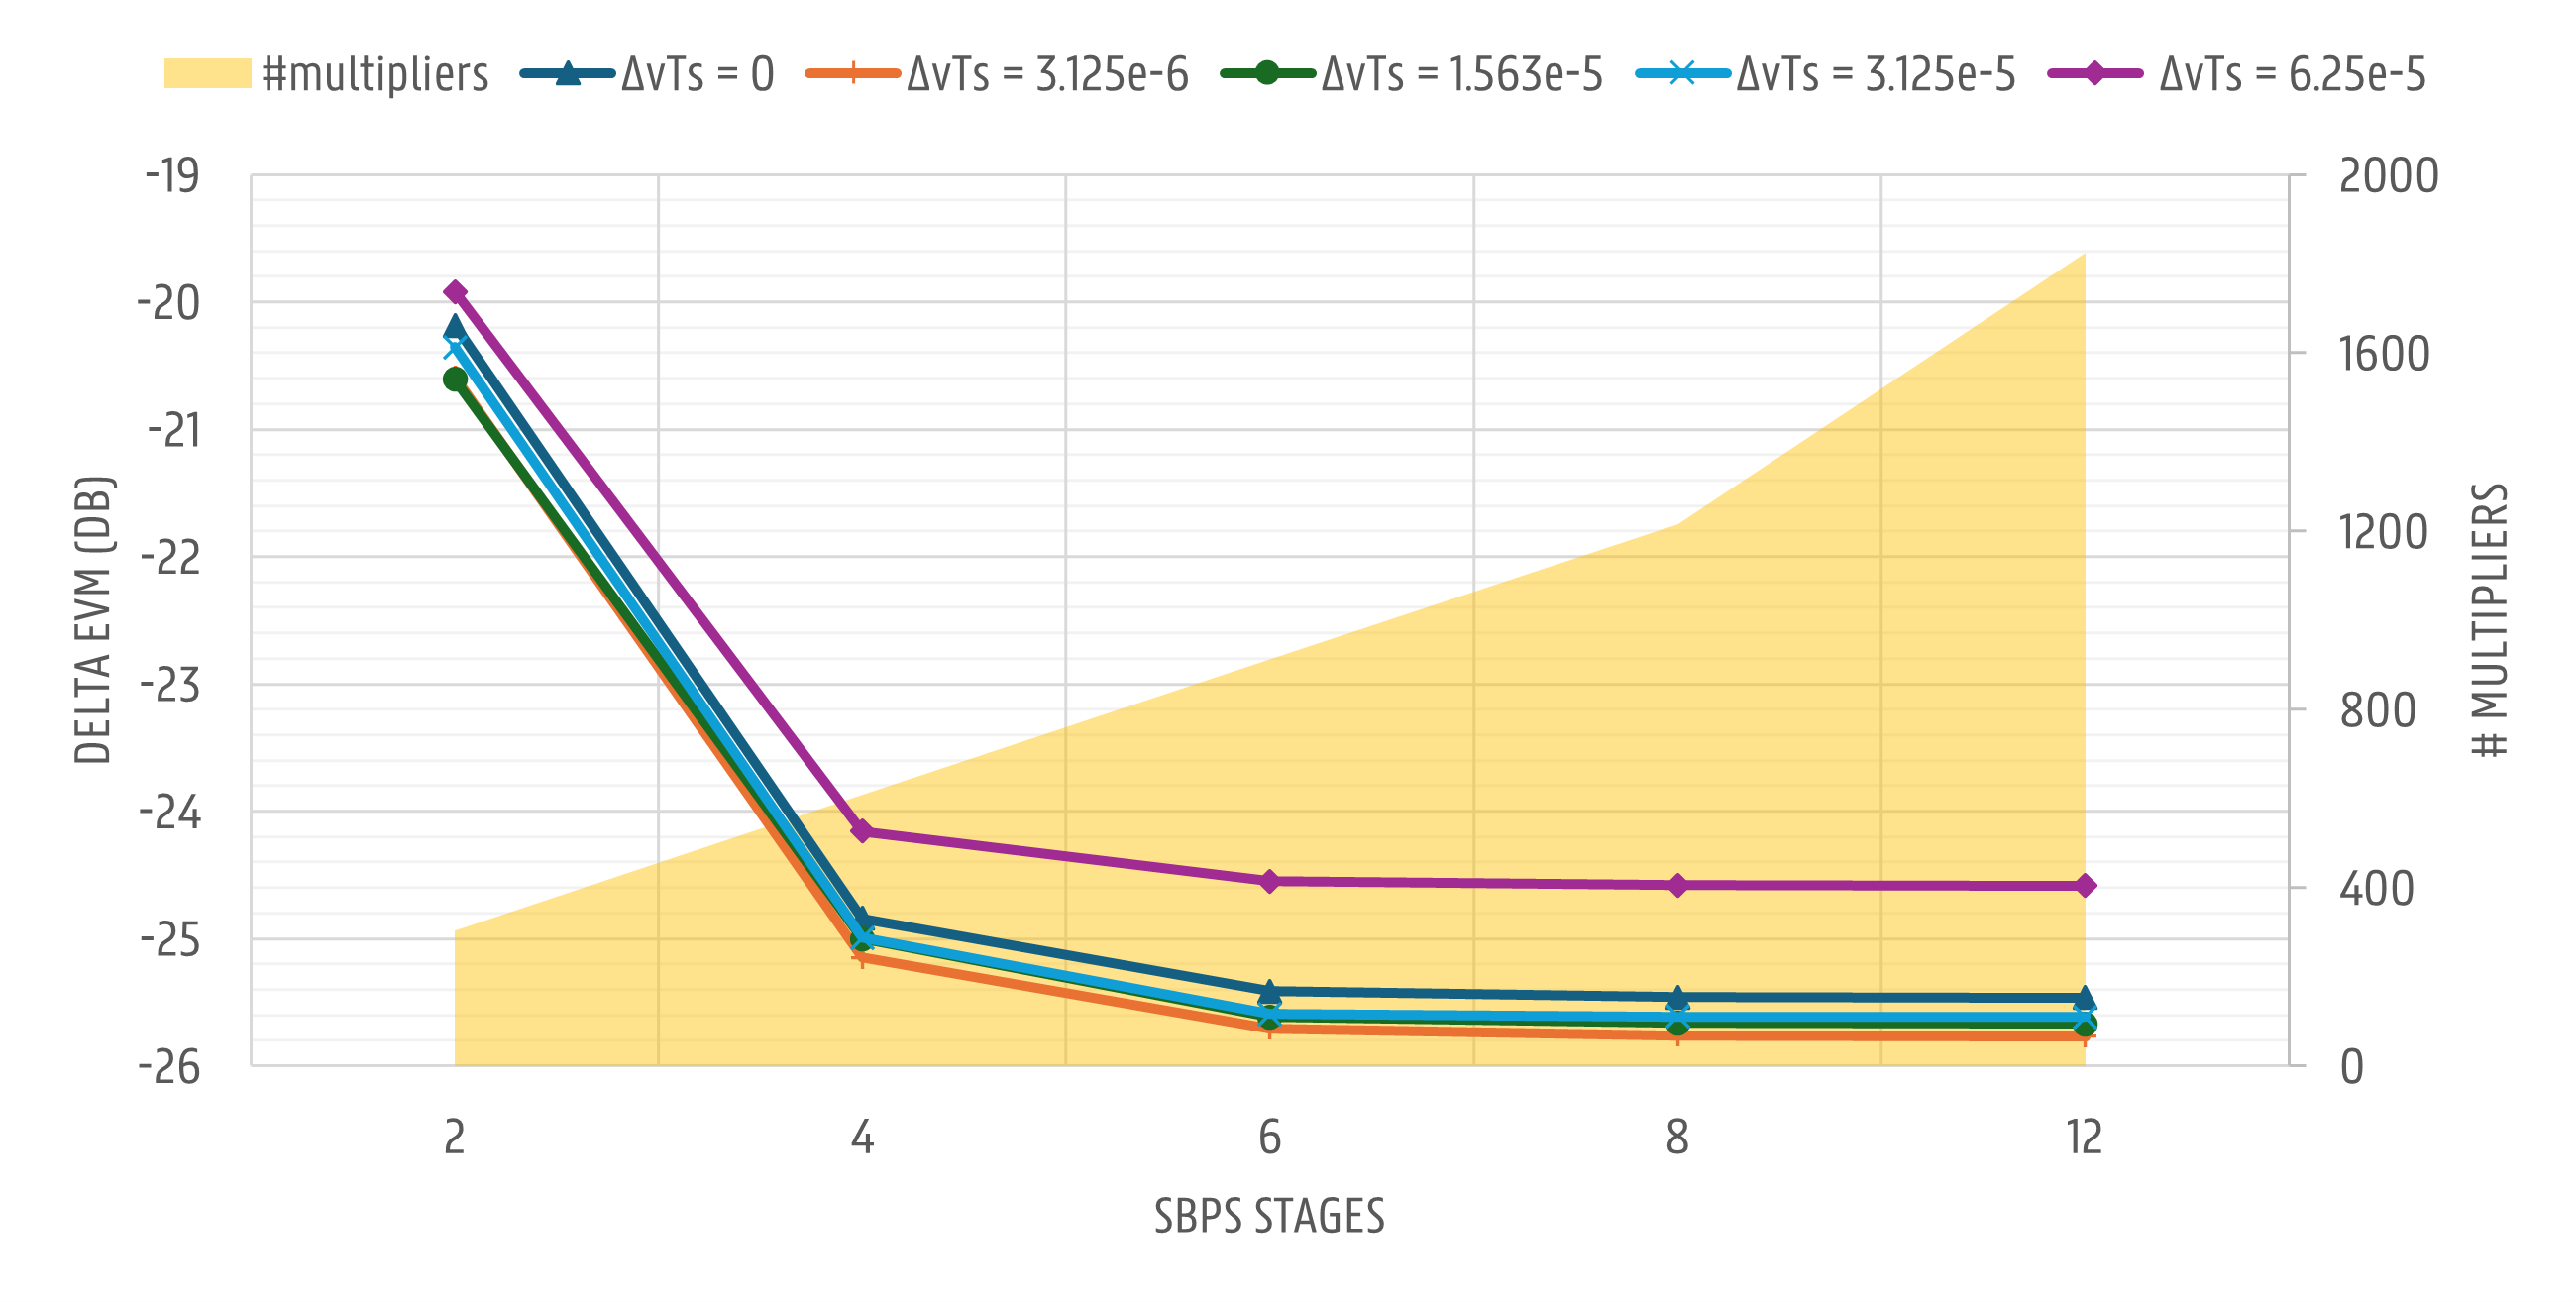
\includegraphics[width=1\linewidth]{figures/SBPSstages_vs_dEVM_linewidth.png}
\caption{Effect of SBPS refinement depth on recovery performance}
\label{fig:results-ber-stages-cfo}
\end{figure}

The strongest improvement occurs when increasing the search depth from two to four stages. With only two stages, the phase estimate is still too coarse, so the recovered \ac{EVM} remains limited by phase quantisation in the \ac{SBPS} estimate. Four stages already move the operating point close to the final performance region. Increasing the depth from four to six stages still gives a measurable improvement, but the gain is smaller. Beyond six stages, the curves are almost flat for all linewidths in the sweep.

This saturation is consistent with the role of the \ac{SBPS} block in the complete architecture. Once the centre-phase estimate is sufficiently accurate, the dominant remaining errors no longer come from the \ac{SBPS} search resolution. They are instead caused by additive noise, linewidth-induced phase variation, spread-estimation error and the finite granularity of the compensation sections. Adding more \ac{SBPS} stages then increases the number of multipliers in the serialized chain without producing a proportional improvement in $\Delta\mathrm{EVM}_{\mathrm{dB}}$.

The linewidth dependence follows the same interpretation. The largest linewidth case remains worse than the lower-linewidth cases over the full stage sweep, because the local phase evolution becomes less well described by the deterministic centre-phase estimate plus a linear spread estimate. This effect cannot be removed by making the centre-phase search indefinitely fine.

\subsection{Influence of compensation sections}

The number of phase-compensation sections controls how finely the estimated spread is applied across one block. Figure~\ref{fig:results-evm-sections-cfo} shows $\Delta\mathrm{EVM}_{\mathrm{dB}}$ versus the number of sections for a fixed residual \ac{CFO} of $\Delta f T_s = 2\times10^{-3}$ and several linewidth settings. The one-section case represents pure blockwise compensation: the whole block is corrected with the unwrapped \ac{SBPS} centre phase, and the spread estimate does not create an intra-block phase profile.

\begin{figure}[H]
\centering
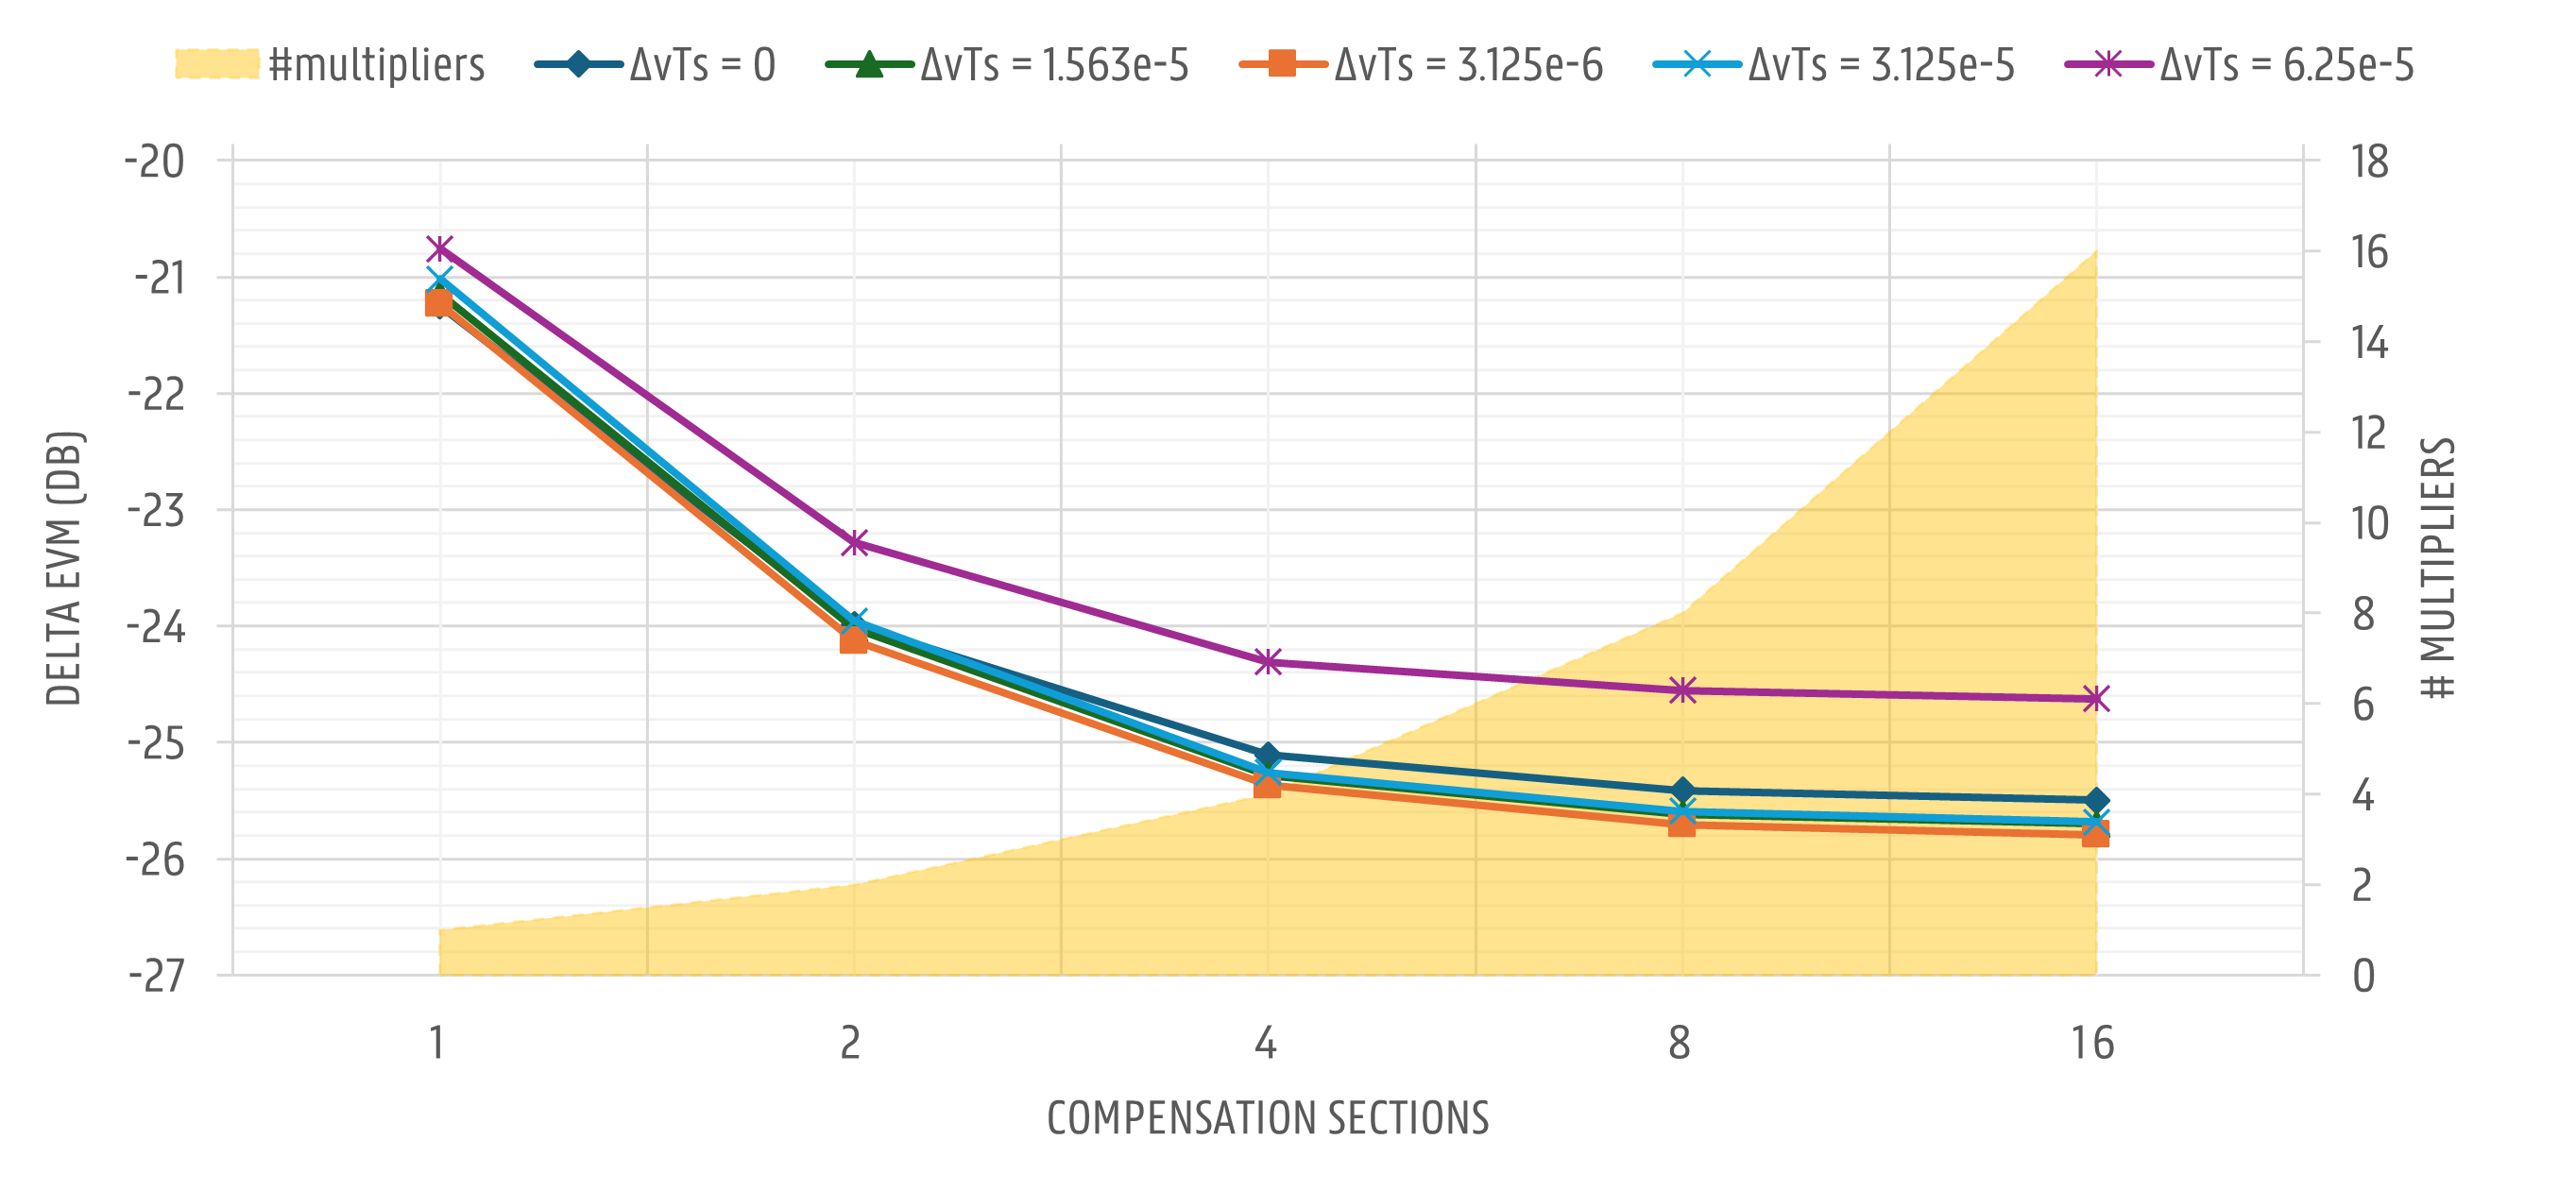
\includegraphics[width=1\linewidth]{figures/compsec_vs_dEVM_ΔfTs​=2e-3.png}
\caption{Effect of phase-compensation granularity on the recovery performance}
\label{fig:results-evm-sections-cfo}
\end{figure}

Increasing the number of sections improves the recovery performance over the full linewidth range. This follows directly from the section-based compensation model in Equation~\ref{eq:section-residual-error}: for an approximately linear phase ramp, smaller sections reduce the maximum residual phase error left inside each section. The largest gain is obtained when moving from one section to two and then to four sections. After this point, the curves begin to saturate. The eight- and sixteen-section configurations still improve the result slightly, but the improvement is much smaller than the cost increase suggested by the multiplier-count trend.

The linewidth trend is also visible in this sweep. The $\Delta\nu T_s = 0$ case, where only the deterministic residual \ac{CFO} is present, obtains the best compensation result. As the linewidth increases, the recovered \ac{EVM} worsens for every section count. This is expected from Equation~\ref{eq:SE-linear-assumption}: the spread estimator and section compensator assume that the phase trajectory inside one block is well approximated by a local linear model. A larger linewidth adds more stochastic, non-linear phase variation inside the block, so increasing the number of deterministic compensation sections cannot remove all of the remaining error.

% \subsection{Block-size trade-off}

% Changing the block size affects both noise averaging in the decision-directed metric and the amount of phase evolution that must be represented inside one block. Figure~\ref{fig:results-block-size} should therefore compare \ac{EVM}, residual phase spread or \ac{BER} for the final block-size candidates. This subsection should be kept short if only one block size is used in the final hardware configuration.

% \begin{figure}[H]
% \centering
% \missingfigure{Performance versus block size for the final stage and section settings.}
% \caption{Influence of processing-block size on carrier-recovery performance}
% \label{fig:results-block-size}
% \end{figure}

\subsection{Error localisation}

The previous sweeps report one aggregate \ac{EVM} value per configuration. To understand where the remaining error originates, the residual \ac{EVM} is also inspected as a function of the symbol position inside the block. This is especially useful for distinguishing centre-phase errors from intra-block phase-slope errors. A centre-phase error would affect all symbol positions similarly, while insufficient spread compensation should mainly affect the block edges.

\begin{figure}[H]
\centering
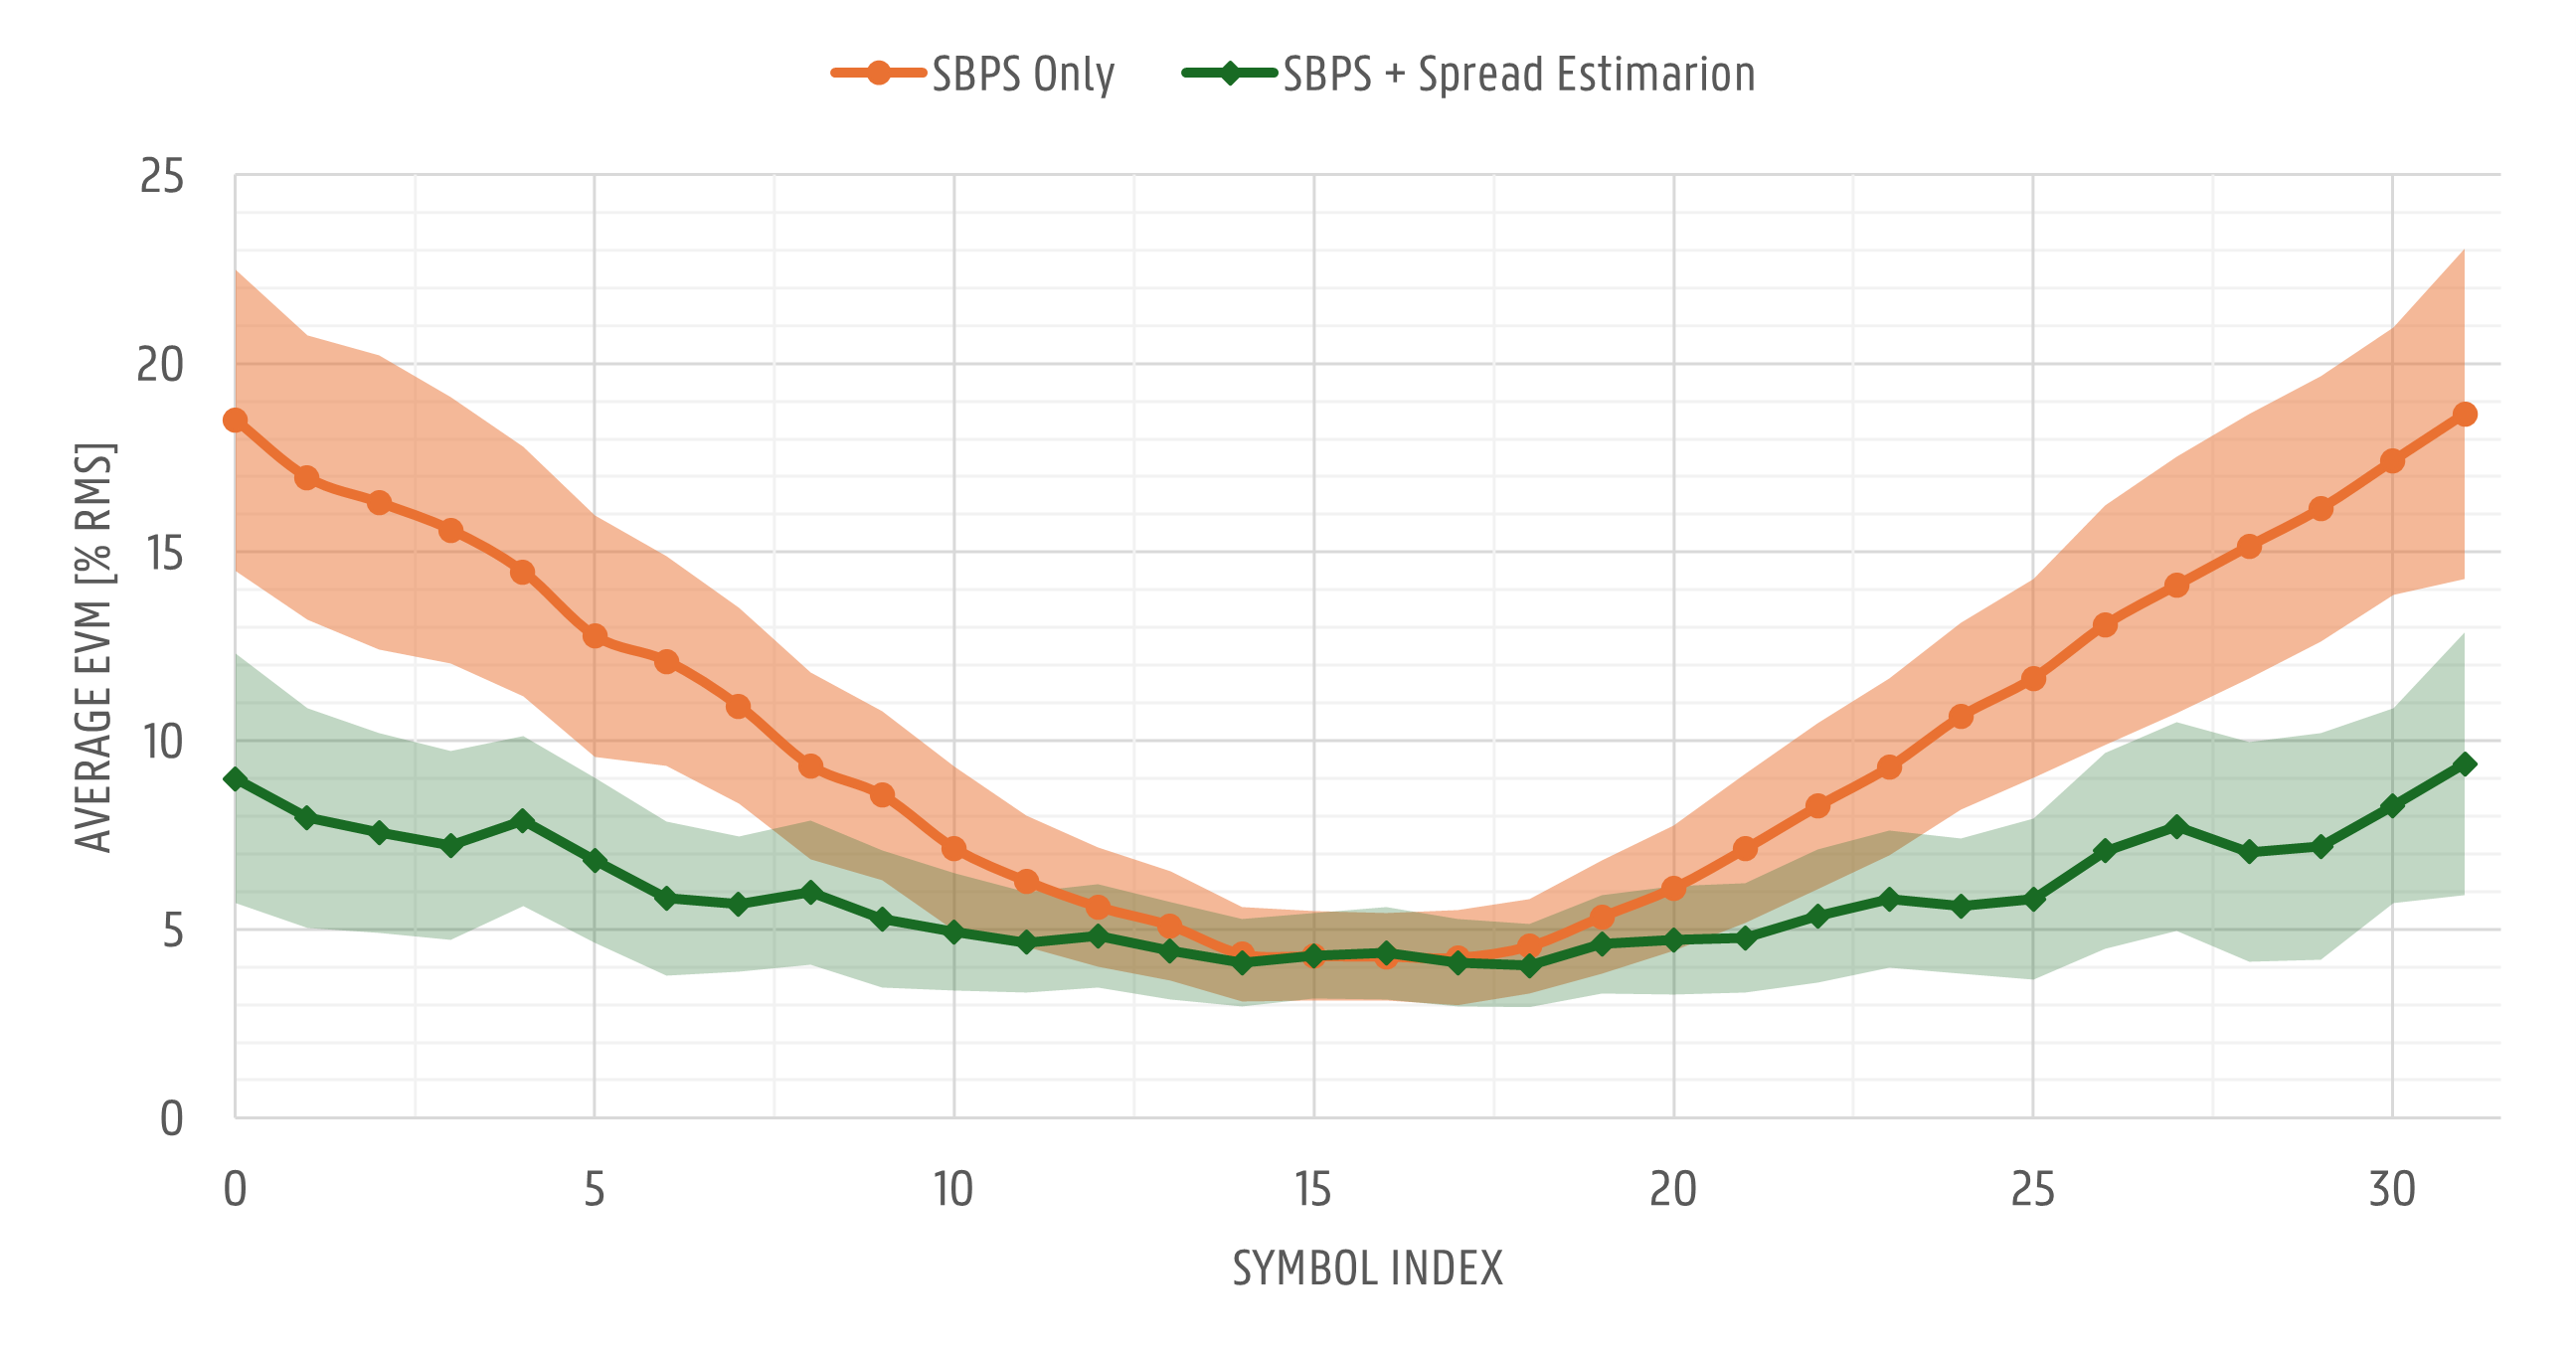
\includegraphics[width=1\linewidth]{figures/symbol_error_localisation_defaults.png}
\caption{Residual EVM after SBPS correction and SBPS + SE correction}
\label{fig:results-residual-EVM-by-symbol}
\end{figure}

Figure~\ref{fig:results-residual-EVM-by-symbol} shows this localisation for the default case, with shaded regions representing the 95\% CI. With \ac{SBPS}-only correction, the residual \ac{EVM} has a clear U-shaped profile: it is lowest near the centre of the block and increases towards both edges. This matches the expected behaviour of a blockwise centre-phase estimate. The centre of the block is corrected well, while symbols further away from the centre retain more of the uncompensated phase ramp.

After adding spread estimation and section-based compensation, the residual \ac{EVM} becomes both lower and flatter over the block. The largest improvement occurs near the first and last symbols, where the \ac{SBPS}-only correction leaves the largest phase error. Near the centre, the difference between both curves is smaller because the centre-phase estimate is already a good correction there. This confirms the intended division of work between both blocks: \ac{SBPS} establishes the centre phase, while \ac{SE} reduces the edge error caused by intra-block phase evolution.

\begin{figure}[H]
\centering
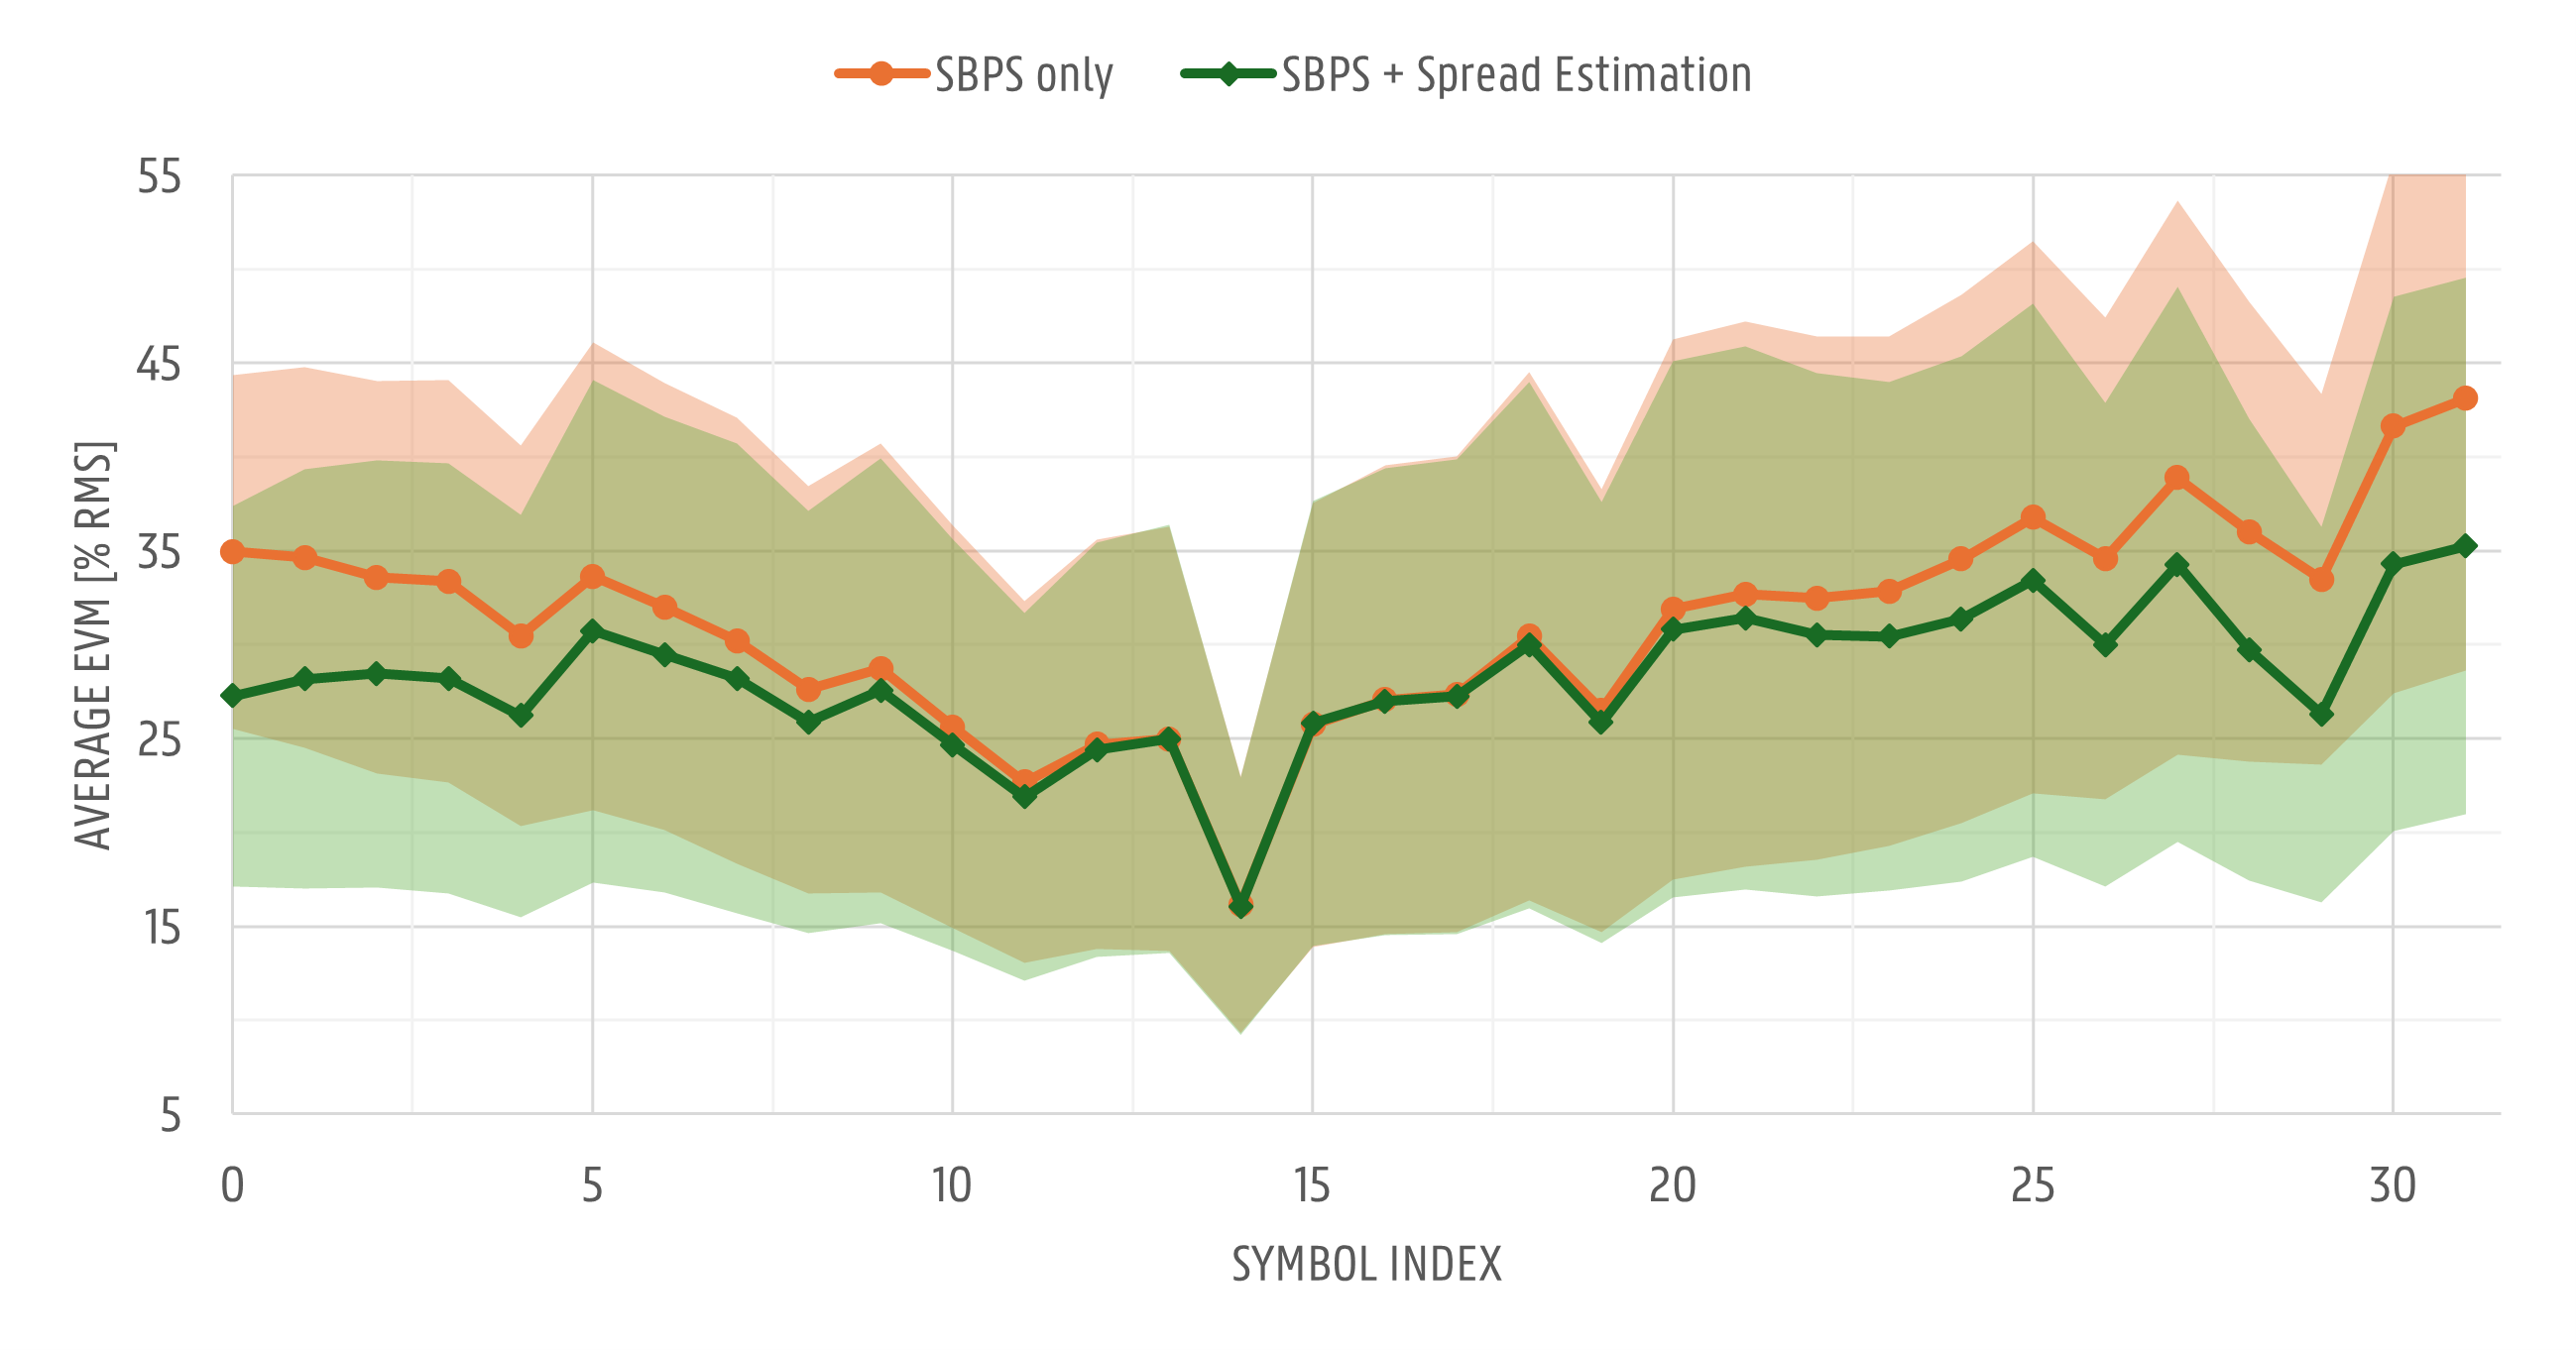
\includegraphics[width=1\linewidth]{figures/symbol_error_localisation_cfo96m_sec16.png}
\caption{Residual EVM after SBPS correction and SBPS + SE correction, 96 MHz CFO}
\label{fig:results-residual-EVM-by-symbol_nondefault}
\end{figure}

Figure~\ref{fig:results-residual-EVM-by-symbol_nondefault} repeats the localisation for a more demanding 96~MHz residual-\ac{CFO} case. At 32~GBd, this corresponds to $\Delta f T_s = 3\times10^{-3}$, so the deterministic phase slope inside one block is larger than in the default case. The residual \ac{EVM} is substantially higher for both correction methods, and the spread between blocks is also larger. The \ac{SBPS}+\ac{SE} curve still improves the average result compared with \ac{SBPS} only, but the improvement is less clean than in the default case.

This behaviour indicates that the receiver is closer to its practical tracking boundary. The centre of the block still benefits from the \ac{SBPS} estimate, but the larger phase evolution makes the linear spread estimate and the section approximation more sensitive to estimation error and linewidth perturbations. The fact that the \ac{EVM} remains position-dependent even with sixteen sections suggests that the limitation is not only the number of compensation sections; spread-estimation accuracy, unwrap robustness and the validity of the local-linear phase assumption also become important. 


The hardware implementation was described in Chapter~\ref{Hardware Implementation}. The goal here is only to connect the measured performance to resource usage and latency.
For the hardware implementation, the XCU-200-fsgd2104-2-e chip from the Virtex UltraScale+ series was used, with Vivado 2025.1 using the default implementation parameters.

\subsection{Resource usage}

The sweep results show where additional hardware stops giving a significant performance improvement for the default setup. The \ac{SBPS} stage sweep points to six refinement stages as the useful knee of the curve, while the compensation-section sweep shows that eight sections capture most of the section-based improvement. The implementation results in this section therefore focus on this operating region and on the clock target that could be reached after routing.

Two sets of implementation results are relevant. The archived \(B=32\) clock sweep was run with six \ac{SBPS} stages and eight compensation sections. It shows that the design closes timing at \(10~\mathrm{ns}\), but that the same pipeline structure is just too slow for an \(8~\mathrm{ns}\) target. A revisited timing-critical version of the design contains the additional register inserted in the spread-estimation reciprocal-multiplication path, the most critical path.
\begin{table}[H]
\centering
\caption{FPGA resource usage for the evaluated receiver configurations}
\label{tab:results-resource-usage}
\small
\begin{tabular}{p{0.34\linewidth} r r r r r l}
\hline
Configuration & LUT & FF & DSP & BRAM & \(T_{\mathrm{clk}}\) [ns] & Result \\
\hline
\(B=32\), baseline pipeline & 33331 & 36006 & 229 & 4 & 10.0 & pass \\
\(B=32\), baseline pipeline & 33340 & 36006 & 229 & 4 & 8.0 & fail \\
\(B=32\), timing-revised pipeline & 33342 & 36007 & 229 & 4 & 8.0 & pass \\
\hline
\end{tabular}
\end{table}

The table shows that the \(8~\mathrm{ns}\) failure in the archived \(B=32\) sweep is not caused by a large increase in area. The passing \(10~\mathrm{ns}\) point and the failing \(8~\mathrm{ns}\) point use practically the same resources: about \(33.3\mathrm{k}\) LUTs, \(36.0\mathrm{k}\) flip-flops, 229 DSP blocks and four BRAM tiles. The revisited design also has the same resource profile. Relative to the failing \(8~\mathrm{ns}\) sweep point, the routed registered design adds one flip-flop and only two LUTs, while the DSP and BRAM counts remain unchanged. On the XCU200 device this corresponds to approximately \(2.82\%\) of the LUTs, \(1.52\%\) of the registers, \(3.35\%\) of the DSP blocks and \(0.19\%\) of the BRAM tiles.
This also supports the algorithmic choices from Figures~\ref{fig:results-ber-stages-cfo} and~\ref{fig:results-evm-sections-cfo}. Adding \ac{SBPS} stages replicates the two-branch rotate-metric-slice structure for each refinement step, so its cost increases approximately linearly with the number of stages. Adding compensation sections increases the number of section phase values and the amount of parallel rotation hardware required by the phase-correction block. Because the measured performance already plateaus around six stages and eight sections, the selected operating point gives a favourable balance between phase-recovery performance, area and timing margin.

\subsection{Latency}\label{subsec:results-latency-timing}

The latency and timing results complete the hardware evaluation by showing whether the selected architecture can be clocked at the intended rate after implementation. Two quantities are considered separately. The first is the pipeline latency, expressed in clock cycles from the assertion of \texttt{in\_valid} for one input block to the corresponding output-valid pulse. This value is fixed by the register structure described in Chapter~\ref{Hardware Implementation}. The second is the post-implementation timing margin reported by Vivado for a selected clock period. This value depends on placement, routing and the selected receiver parameters.

The clock-sweep flow is used to evaluate the design over a small set of candidate clock periods. For each point in the sweep, Vivado is run through implementation and timing analysis using the same \ac{RTL} configuration and device target. The main timing quantities extracted from the implementation reports are the worst negative slack (\texttt{WNS}), total negative slack (\texttt{TNS}), worst hold slack (\texttt{WHS}), total hold slack (\texttt{THS}) and the number of failing setup and hold endpoints. The setup timing condition is considered closed when \texttt{WNS} is non-negative and \texttt{TNS} is zero. Similarly, hold timing is considered closed when \texttt{WHS} is non-negative and \texttt{THS} is zero.

\begin{equation}
    \mathrm{timing~closed}
    =
    (\mathrm{WNS} \geq 0)
    \land
    (\mathrm{TNS} = 0)
    \land
    (\mathrm{WHS} \geq 0)
    \land
    (\mathrm{THS} = 0).
    \label{eq:results-timing-closure}
\end{equation}

For a passing implementation point, the clock frequency is obtained from the constrained clock period:
\begin{equation}
    f_{\mathrm{clk}} = \frac{1}{T_{\mathrm{clk}}}.
    \label{eq:results-clock-frequency}
\end{equation}
% The highest passing clock frequency in the sweep is used as the conservative reported operating point. If adjacent passing and failing periods are available, the limiting period can also be interpreted from the critical-path slack, but the result is still reported as a measured post-route timing point rather than as an extrapolated value.

\begin{table}[H]
\centering
\caption{Post-implementation timing-closure summary for the clock sweep}
\label{tab:results-timing-closure}
\small
\setlength{\tabcolsep}{3pt}
\begin{tabular}{@{}p{0.24\linewidth} r r r r r r r r r l@{}}
\hline
Configuration & \(B\) & \(T_{\mathrm{clk}}\) [ns] & Stages & Sections & \texttt{WNS} [ns] & \texttt{TNS} [ns] & \texttt{WHS} [ns] & \texttt{THS} [ns] & Fail EP & Status \\
\hline
\(B=32\), baseline pipeline & 32 & 10.0 & 6 & 8 & +1.199 & 0.000 & +0.030 & 0.000 & 0/0 & pass \\
\(B=32\), baseline pipeline & 32 & 8.0 & 6 & 8 & -0.257 & -6.797 & +0.039 & 0.000 & 32/0 & fail \\
\(B=32\), timing-revised pipeline & 256 & 8.0 & 6 & 8 & +0.064 & 0.000 & +0.040 & 0.000 & 0/0 & pass \\
\hline
\end{tabular}
\end{table}

The unrevisited pipeline confirms that the unregistered reciprocal-multiplication path is close to the \(8~\mathrm{ns}\) target but does not meet it after routing. The \(10~\mathrm{ns}\) point closes with \(1.199~\mathrm{ns}\) of setup slack, while the \(8~\mathrm{ns}\) point fails with \(-0.257~\mathrm{ns}\) WNS and 32 failing setup endpoints. Hold timing is not the limiting factor in either case: the worst hold slack remains positive and \texttt{THS} is zero.

The routed report of the current registered top-level design shows the effect of inserting the additional register in the critical spread-estimation path. The \(8~\mathrm{ns}\) constraint is met with \(0.064~\mathrm{ns}\) WNS and \(0.040~\mathrm{ns}\) WHS, corresponding to a measured post-route operating point of \(125~\mathrm{MHz}\). The worst setup path is still located inside the spread-estimation block, in the signed reciprocal-multiply logic. 

% In the \(B=32\) sweep the limiting path ran from the reciprocal output register \texttt{out\_inv\_reg[3]} to \texttt{q\_reg\_reg[3]}. In the registered top-level design the worst path starts after the inserted DSP-side register \texttt{ARG\_\_19/DSP\_A\_B\_DATA\_INST/CLK} and ends at \texttt{q\_reg\_reg[17]}. Its reported data-path delay is \(7.887~\mathrm{ns}\), consisting of \(5.262~\mathrm{ns}\) logic delay and \(2.625~\mathrm{ns}\) routing delay. The previous failing \(8~\mathrm{ns}\) sweep point had a worst-path delay of \(8.237~\mathrm{ns}\).
But, the added register splits the arithmetic path enough to recover timing closure with almost no resource penalty.

The pipeline latency is reported in both cycles and time. If the implemented receiver latency is \(L\) cycles, the absolute latency at a selected clock period is
\begin{equation}
    t_{\mathrm{lat}} = L T_{\mathrm{clk}}.
    \label{eq:results-absolute-latency}
\end{equation}
This latency does not affect the steady-state throughput when the design accepts one block per input transaction, but it determines the delay between an input block and the corresponding corrected output block. 
% The most important latency consequence of the timing fix is local: one extra register stage is added in the spread-estimation path and the valid/data alignment is adjusted accordingly.

\begin{table}[H]
\centering
\caption{Pipeline-latency summary for the implemented receiver}
\label{tab:results-pipeline-latency}
\small
\setlength{\tabcolsep}{3pt}
\begin{tabular}{@{}p{0.27\linewidth} p{0.18\linewidth} p{0.14\linewidth} p{0.29\linewidth}@{}}
\hline
Path or block & Latency [cycles] & Latency at \(8~\mathrm{ns}\) [ns] & Comment \\
\hline
\ac{SBPS} valid alignment & \(G_{\mathrm{stages}}G_{\mathrm{stage}}\) & configuration dependent & Knee-point for B=32 uses \(6\cdot14\) alignment cycles. \\
Spread-estimation synchronisation delay & 15 & 120 & Includes the additional register in the reciprocal-multiply path. \\
Phase-correction phase/data alignment & 18 & 144 & Delay used to align the corrected phase information with the block samples. \\
Additional timing-fix cost & +1 & +8 & Extra latency relative to the failing \(8~\mathrm{ns}\) baseline path. \\
% Complete receiver wrapper & fixed pipeline & -- & Throughput is unchanged once the valid-driven pipeline is filled. \\
\hline
\end{tabular}
\end{table}

The final interpretation combines these timing results with the performance sweeps from Section~\ref{sec:results-performance-sweeps}. A configuration that improves \(\Delta\mathrm{EVM}_{\mathrm{dB}}\) only slightly but reduces \texttt{WNS} or lowers the fastest passing clock frequency is not attractive for the final architecture. Conversely, the selected six-stage, eight-section \(B=32\) configuration is already close to \(125~\mathrm{MHz}\), and the registered top-level implementation demonstrates that the remaining limit can be removed with a one-cycle local pipeline change. The throughput remains one block per accepted input transaction after pipeline fill, while the absolute latency increases by only \(8~\mathrm{ns}\) at the \(125~\mathrm{MHz}\) operating point.
